\chapter{DESARROLLO DEL PROYECTO}
\newpage
\section{Introducci\'on}
Para llevar a cabo el desarrollo del presente proyecto se ha tomado en cuenta la division del mismo en tres ``sub-proyectos'': El desarrollo del entorno base (\textit{i}CMS), El desarrollo de las extensiones (M\'odulos, Bloques y Temas) y por \'ultimo el desarrollo de un Framework de soporte a \textit{i}CMS (Framework Jhaley).\\

A continuaci\'on se detallan los aspectos m\'as destacados de cada ``sub-proyecto''.

\section{\textit{i}CMS}
El proyecto iCMS no sigue una metodolog\'ia de desarrollo en particular, por lo tanto este cap\'itulo muestra los elementos utilizados tanto para el desarrollo mismo del proyecto como tambi\'en parte de los resultados obtenidos (modelos).\\

El desarrollo del proyecto fue basado en una lista de tareas para poder conseguir la arquitectura inicial del \textit{i}CMS.\\

\subsection{Lista de tareas}
La lista de tareas que se muestran a continuaci\'on sirvio de base para poder desarrollar el \textit{i}CMS.

\begin{itemize}
\item Definir estructura de Directorios y Archivos.
\item Definir configuraciones b\'asicas.
\item Desarrollar renderizador para las plantillas.
\item Dise\~nar estructura de los m\'odulos y bloques.
\item Desarrollar renderizador para m\'odulos y bloques.
\item Desarrollar clases Singleton (Request, DBO, Factory, Editor WYSIWYG).
\item Desarrollar bloque de menus.
\item Desarrollar bloque de usuarios (pantalla de acceso - login)
\item Desarrollar modulo de contenido.
\item Desarrollar modulo de usuarios (formulario de registro, modificación de datos).
\item Crear librerías de “drag and drop” personalizadas y generalizadas para cualquier tipo de contenido (artículos, bloques, etc.).
\end{itemize}

Durante el desarrollo de estas tareas, han ido surgiendo nuevas tareas m\'as especializadas.

\begin{itemize}
\item Desarrollar m\'odulo de men\'us.
\item Desarrollar bloque de navegaci\'on (breadcrumb).
\item Desarrollar bloque y m\'odulo de noticias.
\item Mejorar el renderizador de plantillas para soportar el reordenamiento de bloques.
\item Actualizar el renderizador de plantillas para soportar soportar la edici\'on de la plantilla.
\end{itemize}

\subsection{Arquiterctura}
Para dise\~nar la arquitectura del sistema \textit{i}CMS se considerar\'on dos patrones arquitect\'onicos, el patr\'on MVC (Modelo-Vista-Controlador) y el patr\'on MVP (Modelo-Vista-Presentador).\\

Mucho de este patr\'on se ven en los distintos m\'odulos que componen el \textit{i}CMS, tambi\'en vemos otros patrones presentes en el desarrollo del proyecto (Singleton, Factory Method).\\

A continuaci\'on se presenta un peque\~no ejemplo sin el patr\'on MVC y luego el mismo ejemplo pero aplicando el patr\'on MVC y el patr\'on MVP:\\

Como se puede apreciar en el siguiente ejemplo, todos los elementos de la aplicaci\'on estan mezclados en un solo archivo.

\begin{lstlisting}[label=mvc_all_in_one,caption=Ejemplo sin ning\'un patr\'on,language=PHP]
<?php 
$db = new PDO('mysql:host=localhost;dbname=bd', 'root', 'password');	
$consulta = $db->prepare('SELECT * FROM items');
$consulta->execute();
$items = $consulta->fetchAll();
?>
<div>
    <table class="adminlist" cellspacing="1">
    	<thead>
        	<tr>
				<th class="title">ID</th>
                <th nowrap="nowrap">Nombre</th>
                <th nowrap="nowrap">Descripcio^oacute<n</th>
            </tr>
        </thead>
        <tbody>
        	<?php foreach ($items as $row) {
        	$link = 'index.php?accion=alguna_accion&id='. $row->id;
        	?>
            <tr>
                <td><?php echo $row->id; ?></td>
                <td><a href="<?php echo $link; ?>"><?php echo $row->nombre; ?></a></td>
                <td><a href="<?php echo $link; ?>"><?php echo $row->descripcion; ?></a></td>
            </tr>
            <?php } ?>
        </tbody>
    </table>
</div>
\end{lstlisting}


El patr\'on MVC separa los elementos de una aplicacion en tres grupos (Modelos, Vistas y Controladores).\\

El controlador es el elemento que se encarga de gestionar todas los eventos que son generados por el usuario a trav\'es de las Vistas, as\'i como tambi\'en de generar las vistas que son el resultado de dichas acciones.

\begin{lstlisting}[label=mvc_controlador,caption=Clase Controlador,language=PHP]
<?php

class Controlador {
	
	public function mostrar(){
		$vista = new Vista();
		$vista->setPlantilla('principal');
		$vista->mostrar();
	}
}
?>
\end{lstlisting}


El modelo es el elemento encargado de la gesti\'on de los datos (almacenamiento y recuperaci\'on).

\begin{lstlisting}[label=mvc_modelo,caption=Clase Modelo,language=PHP]
<?php

class Modelo {
	protected $db;
	public function __construct() {
		$this->db = new PDO('mysql:host=localhost;dbname=bd', 'root', 'password');	
	}
	
	public function getDatos(){
		$consulta = $this->db->prepare('SELECT * FROM items');
		$consulta->execute();
		return $consulta->fetchAll();
	}
}
?>
\end{lstlisting}


La vista es el elemento encargado de estructurar los datos recuperados para presentarlos al usuario, la vista conoce la existencia del modelo y puede interactuar con el.

\begin{lstlisting}[label=mvc_vista,caption=Clase Vista,language=PHP]
<?php
class Vista {
	protected $layout;
    public function mostrar(){
    	$model = new Modelo();
    	$items = $model->getDatos();
    	require 'plantillas/' . $layout . '.php';
    }

	public function setLayout($_layout = ''){
    	$this->layout = $_layout;
    }
}
?>
\end{lstlisting}


La plantilla es un elemento auxiliar de la vista, no es una clase, sino un archivo html con el m\'inimo que sirve para maquetar los datos obtenidos en la vista.

\begin{lstlisting}[label=mvc_plantilla,caption=Plantilla de la vista,language=HTML]
<html>
	<head></head>
	<body>
		<div>
		    <table class="adminlist" cellspacing="1">
    			<thead>
		        	<tr>
						<th class="title">ID</th>
                		<th nowrap="nowrap">Nombre</th>
		                <th nowrap="nowrap">Descripcio^oacute<n</th>
        		    </tr>
		        </thead>
        		<tbody>
		        	<?php foreach ($items as $row) {
        			$link = 'index.php?accion=alguna_accion&id='. $row->id;
		        	?>
        		    <tr>
                		<td><?php echo $row->id; ?></td>
		                <td><a href="<?php echo $link; ?>"><?php echo $row->nombre; ?></a></td>
        		        <td><a href="<?php echo $link; ?>"><?php echo $row->descripcion; ?></a></td>
		            </tr>
        		    <?php } ?>
		        </tbody>
		    </table>
		</div>
	</body>
</html>
\end{lstlisting}


El patr\'on MVP separa (al igual que el patr\'on MVC) los elementos de una aplicaci\'on en tres grupos (Modelos, Vistas y Presentadores). La mayor diferencia entre MVC y MVP es que en el patr\'on MVP, la Vista no sabe de la existencia del Modelo, algo que no sucede en el patr\'on MVC.\\

El presentador es b\'asicamente un controlador, pero no delega la responsabilidad de procesar la informaci\'on que llega ya sea desde la vista o del modelo.

\begin{lstlisting}[label=mvp_presentador,caption=Clase Presentador,language=PHP]
<?php
class Presentador {
	public function mostrar(){
		$modelo = new Modelo();
		$items = $modelo->getDatos();
		require 'principal.php';
	}
}
?>
\end{lstlisting}


El modelo trabaja de la misma forma que en el patr\'on MVC.

\begin{lstlisting}[label=mvp_modelo,caption=Clase Modelo,language=PHP]
<?php

class Modelo {
	protected $db;
	public function __construct() {
		$this->db = new PDO('mysql:host=localhost;dbname=bd', 'root', 'password');	
	}
	
	public function getDatos(){
		$consulta = $this->db->prepare('SELECT * FROM items');
		$consulta->execute();
		return $consulta->fetchAll();
	}
}
?>
\end{lstlisting}


La vista es el elemento encargado de estructurar los datos recuperados por el presentador para mostrarlos al usuario.

\begin{lstlisting}[label=mvp_vista,caption=Vista,language=HTML]
<html>
	<head></head>
	<body>
		<div>
		    <table class="adminlist" cellspacing="1">
    			<thead>
		        	<tr>
						<th class="title">ID</th>
                		<th nowrap="nowrap">Nombre</th>
		                <th nowrap="nowrap">Descripcio^oacute<n</th>
        		    </tr>
		        </thead>
        		<tbody>
		        	<?php foreach ($items as $row) {
        			$link = 'index.php?accion=alguna_accion&id='. $row->id;
		        	?>
        		    <tr>
                		<td><?php echo $row->id; ?></td>
		                <td><a href="<?php echo $link; ?>"><?php echo $row->nombre; ?></a></td>
        		        <td><a href="<?php echo $link; ?>"><?php echo $row->descripcion; ?></a></td>
		            </tr>
        		    <?php } ?>
		        </tbody>
		    </table>
		</div>
	</body>
</html>
\end{lstlisting}


Dadas las enormes similitudes entre estos dos patrones, se decidi\'o hacer uso del patr\'on MVC, la raz\'on para esta elecci\'on es que todas las extensiones tienen caracteristicas similares pero no iguales a las de Joomla, con lo cual se plantea para un futuro brindar el soporte necesario para que \textit{i}CMS sea totalmente compatible con las extensiones de Joomla.\\

\subsection{Modelo de Clases}
Como ya fue citado en el marco referencial, el modelo clases es la herramienta que da soporte, de alguna manera a la Programaci\'on Orientada a Objetos. Representando a los objetos que son participes del de sistema \textit{i}CMS.\\
A continuaci\'on podemos ver el modelo de clases general del proyecto \textit{i}CMS.

\newpage
\begin{figure}[h]
\centering
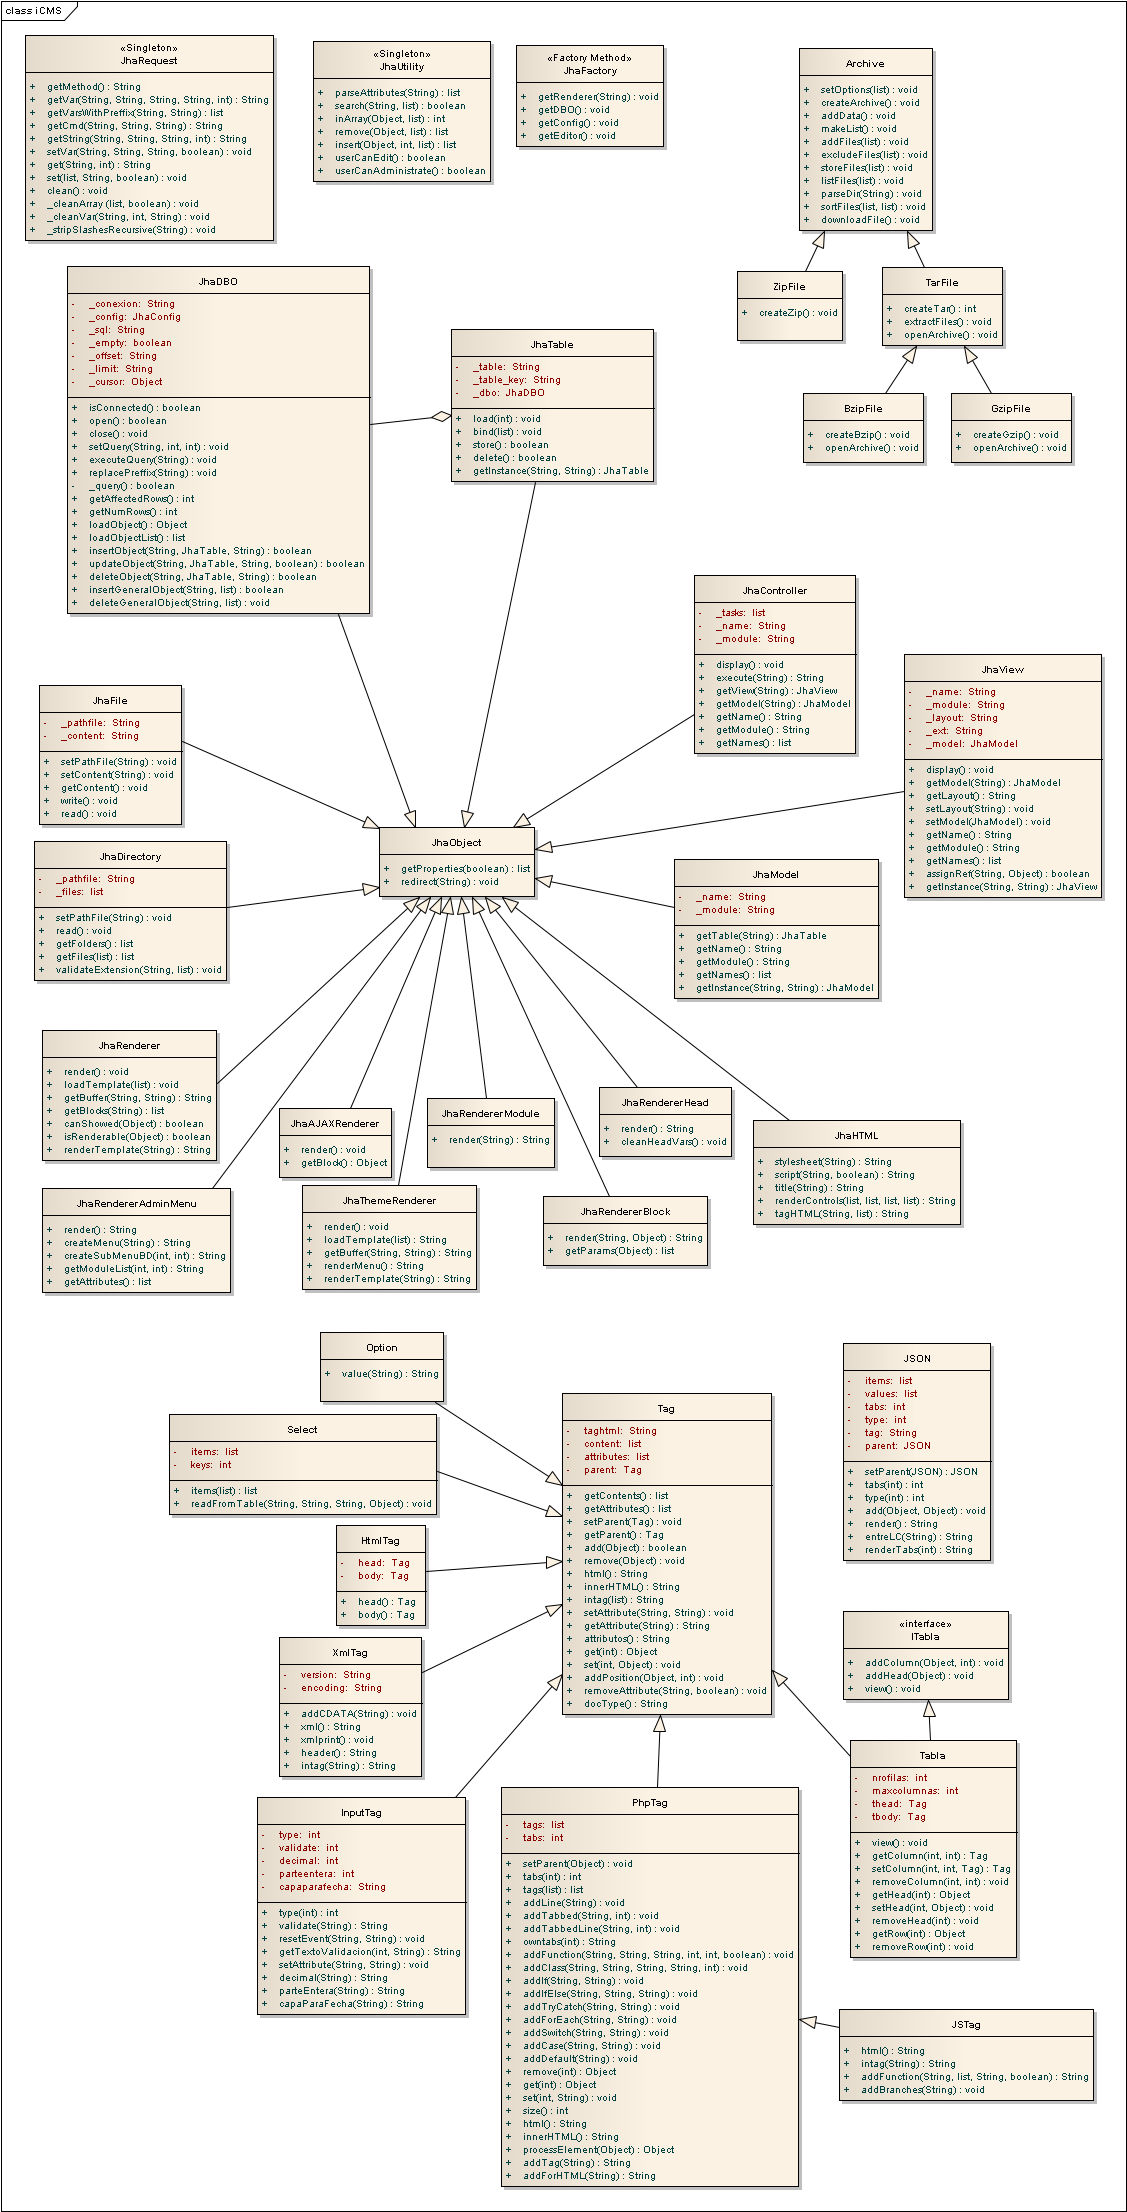
\includegraphics[scale=.24, keepaspectratio=true]{imagenes/03_imagen.png}
\caption{Modelo de clases general. [Elaboraci\'on propia].}
\end{figure}
\clearpage
\newpage

\subsubsection{Aplicaci\'on de los patrones \textit{Singleton} y \textit{Factory Method}}
La aplicaci\'on de estos patrones en el sistema se da en tres clases que son utlizadas por todo el sistema, desde el \textit{Framework Jhaley} hasta las extensiones (m\'odulos y bloques).\\

\begin{figure}[h]
\centering
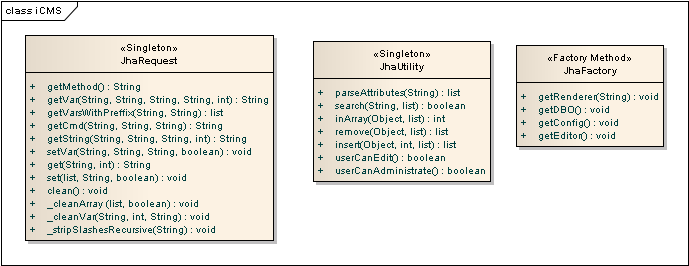
\includegraphics[scale=.5, keepaspectratio=true]{imagenes/04_imagen.png}
\caption{Modelo de clases: Patrones Singleton y Factory Method. [Elaboraci\'on propia].}
\end{figure}

La clase \emph{JhaFactory} es la encargada de crear las instancias Singleton, si la instancia ya existe, entonces esta es reutilizada.

\begin{lstlisting}[label=factory_method,caption=Clase Factory Method]
<?php 
defined( '_JHAEXEC' ) or die( 'Access Denied' );
jhaimport('jhaley.base.object');

class JhaFactory extends JhaObject {
    static function &getRenderer($type = null){
        static $renderer;
       	if($type == null){
       		if(JhaRequest::getVar('elem') == 'mod_base' && JhaRequest::getVar('controller') == 'theme' && (JhaRequest::getVar('task') == 'personalizeTheme' || JhaRequest::getVar('task') == 'savePersonalizedChanges')){
       			jhaimport('jhaley.html.theme'); 
	            $renderer = new JhaThemeRenderer();
       		}
       		else {
	            jhaimport('jhaley.html.renderer'); 
	            $renderer = new JhaRenderer();
       		}
       	}
       	elseif($type == 'block'){
       		jhaimport('jhaley.html.block'); 
            $renderer = new JhaRendererBlock();
       	}
       	elseif($type == 'module'){
            .....
        }
        return $renderer;
    }
    
	static function &getDBO(){
        static $dbo;
        if (!is_object($dbo)) {
            jhaimport('jhaley.db.dbo');             
            $dbo = new JhaDBO(JhaFactory::getConfig());
        }
        return $dbo;
    }
    
	static function &getConfig(){
        static $config;
        if (!is_object($config)) {
            require_once JHA_CONFIGURATION_PATH . DS . 'config.php'; 
            $config = new JhaConfiguration();
        }
        return $config;
    }

	.....
}
?>
\end{lstlisting}


Un ejemplo claro del uso del patr\'on Singleton se puede ver en la instancia de la clase \emph{JhaDBO}, la cual es utilizada constantemente en los modelos de los distintos m\'odulos.

\begin{lstlisting}[label=singleton,caption=Patr\'on Singleton en acci\'on]
<?php
defined( '_JHAEXEC' ) or die( 'Access Denied' );
jhaimport('jhaley.mvc.model');

class MenuModelMenu extends JhaModel {
    public function __construct() {
        parent::__construct();
    }
    
    public function getMenus(){
    	$db = &JhaFactory::getDBO();
        $db->setQuery('SELECT m.id, m.titulo, m.descripcion, u.nombre as creador FROM #__menu as m, #__usuario as u WHERE m.usuario = u.id ORDER BY m.id');
        return $db->loadObjectList();
    }
    
	public function getMenu($id){
    	$db = &JhaFactory::getDBO();
        $db->setQuery('SELECT * FROM #__menu WHERE id = ' . $id);
        return $db->loadObject();
    }
    .....
}
?>
\end{lstlisting}


\subsubsection{Manejo de Archivos compresos}

\begin{figure}[h]
\centering
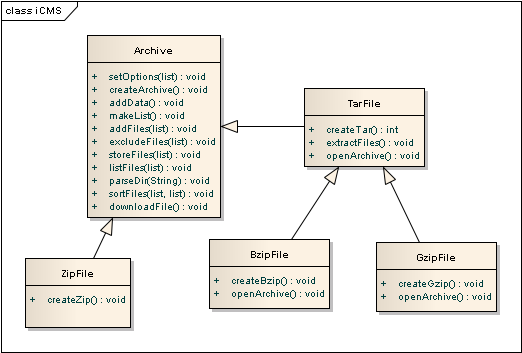
\includegraphics[scale=.4, keepaspectratio=true]{imagenes/05_imagen.png}
\caption{Modelo de clases: Manejo de Archivos Compresos. [Elaboraci\'on propia].}
\end{figure}

El manejo de archivos compresos esta dado por un grupo de clases especializadas para este cometido, adem\'as estas clases utilizan elementos propios del core de PHP a trav\'es de la manipulaci\'on de los archivos compresos en forma de datos binarios.\\

La superclase \textit{Archive} contiene ciertos elementos que merecen ser detallados.\\

Una de las caractiristicas primordiales es que sus configuraciones est\'an dadas por una serie de opciones:
\begin{itemize}
	\item[\textbf{basedir}], describe el directorio donde se comprimir\'an/descomprimir\'an los archivos.
	\item[\textbf{name}], describe el nombre del archivo compreso.
	\item[\textbf{inmemory}], describe se se manipulara el archivo directamente desde el disco duro o en memoria.
	\item[\textbf{level}], describe el nivel de compresi\'on.
	\item[...] entre otros.
\end{itemize}

\begin{lstlisting}[label=compress_option,caption=Opciones para la configuraci\'on de los compresos.]
<?php
defined( '_JHAEXEC' ) or die( 'Access Denied' );

class Archive {
	function __construct($name) {
		$this->options = array (
			'basedir' => ".",
			'name' => $name,
			'prepend' => "",
			'inmemory' => 0,
			'overwrite' => 0,
			'recurse' => 1,
			'storepaths' => 1,
			'followlinks' => 0,
			'level' => 3,
			'method' => 1,
			'sfx' => "",
			'type' => "",
			'comment' => ""
		);
		$this->files = array ();
		$this->exclude = array ();
		$this->storeonly = array ();
		$this->error = array ();
	}
    .....
}
?>
\end{lstlisting}


Otra caracter\'istica es la posibilidad de crear archivos descargables desde los navegadores.

\begin{lstlisting}[label=compress_downloadable,caption=Opciones para la descarga de los compresos.]
<?php
defined( '_JHAEXEC' ) or die( 'Access Denied' );

class Archive {
    .....
    function downloadFile() {
		if ($this->options['inmemory'] == 0) {
			$this->error[] = "Can only use download_file() if archive is in memory. Redirect to file otherwise, it is faster.";
			return;
		}
		switch ($this->options['type']) {
			case "zip":
				header("Content-Type: application/zip");
			break;
			case "bzip":
				header("Content-Type: application/x-bzip2");
			break;
			case "gzip":
				header("Content-Type: application/x-gzip");
			break;
			case "tar":
				header("Content-Type: application/x-tar");
		}
		$header = "Content-Disposition: attachment; filename=\"";
		$header .= strstr($this->options['name'], "/") ? substr($this->options['name'], strrpos($this->options['name'], "/") + 1) : $this->options['name'];
		$header .= "\"";
		header($header);
		header("Content-Length: " . strlen($this->archive));
		header("Content-Transfer-Encoding: binary");
		header("Cache-Control: no-cache, must-revalidate, max-age=60");
		header("Expires: Sat, 01 Jan 2000 12:00:00 GMT");
		print($this->archive);
	}
}
?>
\end{lstlisting}


%Ejemplo Zip y diferencia con Tar
Las clases \emph{ZipFile} y \emph{TarFile} extienden directamente de \emph{Archive}, mientras que \emph{ZipFile} representa a los archivos compresos completamente formados, \emph{TarFile} representa a un archivo de empaquetado.

\begin{lstlisting}[label=compress_zip,caption=Compresos Zip.]
<?php
defined( '_JHAEXEC' ) or die( 'Access Denied' );
jhaimport('jhaley.compress.archive');

class ZipFile extends Archive {
	function __construct($name) {
		parent::__construct($name);
		$this->options['type'] = "zip";
	}

	function createZip() {
		...
	}
}
?>
\end{lstlisting}


\begin{lstlisting}[label=compress_tar,caption=Empaquetadores Tar.]
class TarFile extends Archive {
	function __construct($name) {
		parent::__construct($name);
		$this->options['type'] = "tar";
	}

	function createTar() {
		...
	}
}
?>
\end{lstlisting}


Los compresos \emph{Gzip}, \emph{TGzip}, \emph{Bzip} y \emph{TBzip} son representados por las subclases \emph{GzipFile} y \emph{BzipFile}. Lo que se gana separando en distintas clases el manejo de los compresos son dos cosas. Primero, que se tienen clases especializadas en un solo tipo de compreso a la vez. Segundo, que es mucho m\'as sencillo a\~nadir nuevos tipos de compresos por medio de la herencia y definici\'on del comportamiento del nuevo compreso.

\subsubsection{Clases para la Gesti\'on de la Base de Datos}
Las clases que se ven en el siguiente gr\'afico son escenciales para la gesti\'on de la informaci\'on en la base de datos. La clase \textit{JhaDBO} sigue el patr\'on Singleton y es utilizado en todas las llamadas a la base de datos, la clase JhaTable es la superclase para todos los DTOs (Data Transfer Object) que representan a las tablas de la base de datos.\\

\begin{figure}[h]
\centering
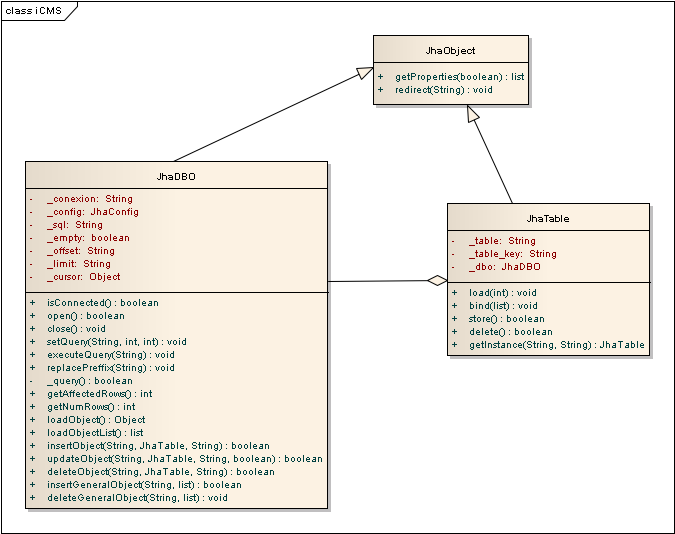
\includegraphics[scale=.5, keepaspectratio=true]{imagenes/06_imagen.png}
\caption{Modelo de clases: Gesti\'on de Base de Datos. [Elaboraci\'on propia].}
\end{figure}

A continuaci\'on se describen brevemente las clases dedicadas a la gesti\'on de base de datos.\\

Todo los objetos de \textit{iCMS} tienen la capacidad de redireccionar a otras URLs, esto es bastante \'util sobre todo en la secci\'on de administraci\'on de \textit{i}CMS, tambi\'en cuentan con la capacidad de recuperar sus propiedades internas de los objetos.\\

\begin{lstlisting}[label=jha_object,caption=Objeto Padre.]
<?php
defined( '_JHAEXEC' ) or die( 'Access Denied' );

class JhaObject{
    public function getProperties( $isPublic = true ) {
        $vars  = get_object_vars($this);
        if($isPublic) {
            foreach ($vars as $key => $value) {
                if ('_' == substr($key, 0, 1)) {
                    unset($vars[$key]);
                }
            }
        }
        return $vars;
    }
    
    protected function redirect($url = 'index.php'){
    	$config = JhaFactory::getConfig();
        if (preg_match( '#^index[2]?.php#', $url )) {
            $host = 'http://' . $_SERVER['HTTP_HOST'];
            $site = $config->site;
            $url = $host . $site . $url;
        }
        header( 'HTTP/1.1 301 Moved Permanently' );
        header( 'Location: ' . $url );
    }
}
?>
\end{lstlisting}


\emph{JhaDBO} es un objeto creado con la \'unica finalidad de procesar y ejecutar las consultas SQL nativas, adicionalmente contiene funciones auxiliares para realizar el trabajo de procesamiento de las consultas.

\begin{lstlisting}[label=jha_dbo,caption=DBO (DataBase Object).]
<?php
...

class JhaDBO extends JhaObject {
	//Conexion a la base de datos
	private $_conexion;
	
	//Configuracion del sitio
	private $_config;
	
	//Consulta SQL 
	private $_sql;
	private $_empty;
	
	//Offset y limit, sirven para obtener resultados parciales.
	private $_offset;
	private $_limit;
	private $_cursor;
	
	function __construct($config = null){
		$this->_config = $config;
		if(!$this->open()){
			throw new Exception ( "Error al conectarse a la Base de Datos." );
		}
	}
	...
	
	/**
	 * Abre una conexion a la base de datos, esta conexion se deberia abrir una sola vez.
	 */
	public function open(){
		...
	}
	
  public function close() {
    ...
  }
    
  public function setQuery($query, $offset = 0, $limit = -1){
  	$this->_sql = $this->replacePreffix($query);
  	$this->_offset = $offset;
  	$this->_limit = $limit;
  }
  
  /**
   * Establece la consulta SQL y luego la ejecuta
   */
  public function executeQuery($query){
  	...
  }
  
  private function replacePreffix($query){
  	return str_replace("#__", $this->_config->db_preffix, $query);
  }
  
  /**
   * Ejecuta la consulta SQL
   */
  private function _query(){
  	...
  }
  ...
  
  /**
   * Tras la ejecucion de la consulta SQL, este metodo retorna el resultado como un Objeto
   */
  public function loadObject() {
    ...
  }
  
  /**
   * Tras la ejecucion de la consulta SQL, este metodo retorna el resultado como una lista de Objetos
   */
  public function loadObjectList( $key = '' ) {
    ...
  }
  
  /**
   * Inserta los datos del objeto en la base de datos.
   */
  public function insertObject( $table, &$object, $keyName = NULL ) {
    ...
  }
  
  /**
   * Actualiza la informacion  de la base da datos con la informacion del objeto
   */
  public function updateObject( $table, &$object, $keyName, $updateNulls = true ) {
    ...
  }
  
  /**
   * Elimina el registro descrito por el objeto
   */
  public function deleteObject( $table, &$object, $keyName = NULL ) {
    ...
  }

  public function insertid() {
    return mysql_insert_id($this->_conexion);
  }
  
  /**
   * Inserta registros en la base de datos con mas de un valor como clave primaria.
   */
  public function insertGeneralObject( $table, $elems) {
    ...
  }
  
  /**
   * Elimina registros de la base de datos que tienen mas de un valor como clave primaria.
   */
  public function deleteGeneralObject( $table, $elems) {
    ...
  }
}
?>
\end{lstlisting}


\subsubsection{Clases para la Gesti\'on de Archivos y Directorios}
Las clases para la gesti\'on de los archivos y directorios se muestran en el siguiente diagrama. La clase \textit{JhaFile} sirve principalmente para la lectura y escritura de archivos, la clase \textit{JhaDirectory} provee una estructura para gestionar los archivos y subdirectorios de un directorio.\\

\begin{figure}[h]
\centering
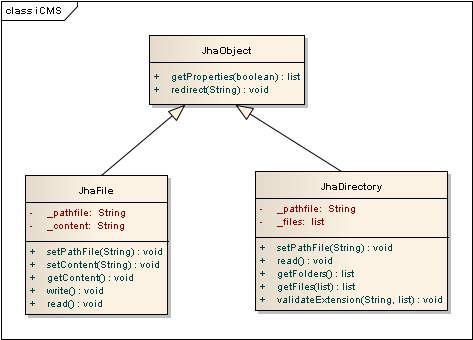
\includegraphics[scale=.5, keepaspectratio=true]{imagenes/07_imagen.png}
\caption{Modelo de clases: Gesti\'on de Archivos y Directorios. [Elaboraci\'on propia].}
\end{figure}

A continuaci\'on se describen brevemente las clases dedicadas a la gesti\'on de archivos y directorios.\\

La clase \emph{JhaFile} permite interactuar de forma directa con los diferentes archivos a trav\'es de sus m\'etodos \emph{read} y \emph{write}.\\

\begin{lstlisting}[label=jha_file,caption=JhaFile.]
<?php
...

class JhaFile extends JhaObject {
	var $_pathfile;
	var $_content;
	
	public function __construct($pathfile = '', $content = ''){
		...
	}
	
	public function setPathFile($pathfile){
		$this->_pathfile = $pathfile;
	}
	
	public function setContent($content){
		$this->_content = $content;
	}
	
	public function getContent(){
		return $this->_content;
	}
	
	/**
	 * Se encarga de escribir el archivo.
	 */
	public function write(){
		...
	}
	
	/**
	 * Se encarga de leer el archivo.
	 */
	public function read(){
		...
	}
}
?>
\end{lstlisting}


La clase \emph{JhaDirectory} se combina con los objetos de tipo \emph{JhaFile} para permitir interactuar tanto con los diferentes archivos como con los directorios a trav\'es de sus m\'etodos \emph{getFolders} y \emph{getFiles}, ademas cuenta con una funci\'on extra para validar las extensiones de los archivos \emph{validateExtension}.\\

\begin{lstlisting}[label=jha_directory,caption=JhaDirectory.]
<?php
...

class JhaDirectory extends JhaObject {
	var $_pathfile;
	var $_files;
	
	public function __construct($pathfile = '.'){
		...
	}
	
	public function setPathFile($pathfile){
		$this->_pathfile = $pathfile;
	}
	
	public function read(){
        $this->_files = scandir($this->_pathfile);
	}
	
	/**
	 * En funcion al filepath recibido, retorna todos los directorios existentes en el.
	 */
	public function getFolders(){
		...
	}
	
	/**
	 * En funcion al filepath recibido, retorna todos los archivos existentes en el.
	 * No toma en cuenta los archivos de los directorios.
	 */
	public function getFiles($filetypes = array()){
		...
	}
	
	/**
	 * Encargado de validar que todos los archivos del directorio tengan la misma extension
	 */
	private function validateExtension($file, $filetypes){
		...
	}
}
?>
\end{lstlisting}


\subsubsection{Clases para la Gesti\'on de Elementos Web}
Las clases para la gesti\'on de los elementos web se muestran en el siguiente diagrama. Estas clases estan basadas en el Framework Goaamb (desarrollado por el Ingeniero de Sistemas Alvaro Michel Barrera).\\
Todas estas clases han sido pensadas principalmente para trabajar con generadores de c\'odigo, pero en el proyecto iCMS se hace uso de ellas principalmente en el manejo de archivos XML y JS.\\

\begin{figure}[h]
\centering
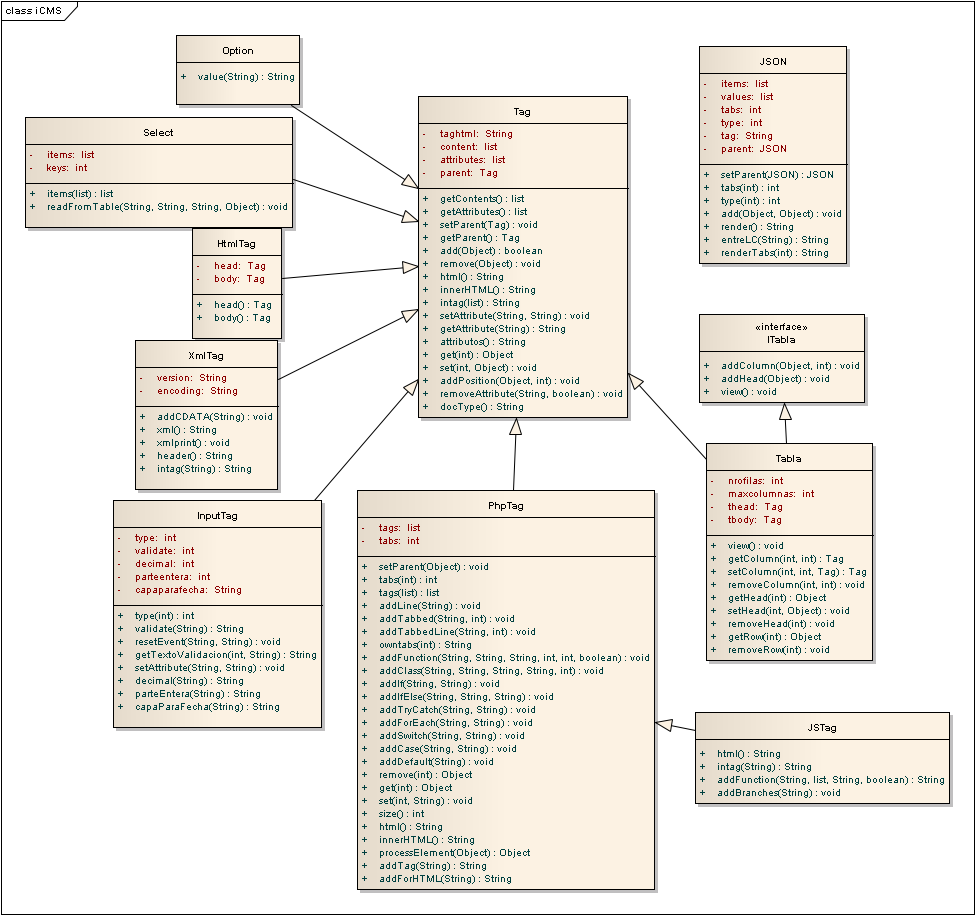
\includegraphics[scale=.4, keepaspectratio=true]{imagenes/08_imagen.png}
\caption{Modelo de clases: Gesti\'on de Elementos Web. [Elaboraci\'on propia].}
\end{figure}

Como podemos ver en la figura anterior, la super clase \emph{Tag} contienen la mayor parte de las funciones propias para los elementos HTML y PHP. Asimismo muchos de los elementos HTML est\'an representados por las clases: \emph{HtmlTag}, \emph{InputTag}, \emph{Select}, \emph{Option} y \emph{Tabla}. Por otro lado tenemos a la clase para el manejo de documentos XML: \emph{XmlTag}. Para el manejo de c\'odigos PHP, tenemos la clase \emph{PhpTag}; dado que los elementos JavaScript tienen cierto parecido con los tags php, la clase JSTag extiende de esta \'ultima.\\
Los elementos JSON se comportan de una manera muy distinta a los elementos que tienen ``tags'', raz\'on por lo cual la clase \emph{JSON} no extiende de ninguna otra.

\subsubsection{Clases de la Arquitectura del \textit{i}CMS}
Las clases que se muestran a continuaci\'on son las superclases que representan al patr\'on Modelo-Vista-Controlador. Las implementaciones de estas superclases estan presentes en las distintas extensiones (m\'odulos).\\

\begin{figure}[h]
\centering
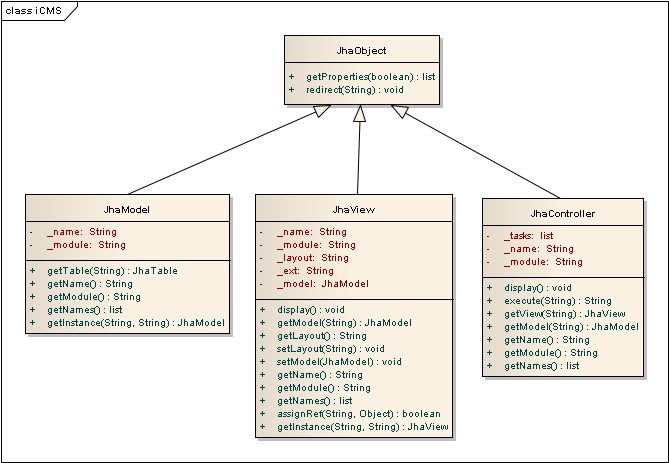
\includegraphics[scale=.65, keepaspectratio=true]{imagenes/09_imagen.png}
\caption{Modelo de clases: Modelo-Vista-Controlador. [Elaboraci\'on propia].}
\end{figure}

La clase \emph{JhaModel} describe dos m\'etodos importantes como \emph{getTable} y \emph{getInstance}; \emph{getTable} se encarga de recuperar objetos de tipo \emph{JhaTable} y es principalmente utilizada a la hora de recuperar registros de la base de datos. Por otro lado \emph{getInstance} retorna una instancia del modelo en cuesti\'on, es decir que depende del m\'odulo desde el que se llame a este m\'etodo.

\begin{lstlisting}[label=jha_model,caption=JhaModel.]
<?php
...

class JhaModel extends JhaObject {
	
	protected $_name;
	protected $_module;
	
    public function __construct(){
        if (empty( $this->_name ) || empty( $this->_module )) {
            $this->_name = $this->getName();
            $this->_module = $this->getModule();
        }
    }
    
    public function &getTable($name = '') {
    	...
    }
    ...
    
    public function &getInstance($name, $prefix){
        ...
    }
}
?>
\end{lstlisting}


La clase \emph{JhaView} se encarga de renderizar las diferentes plantillas dependiendo del controlador y la acci\'on relacionada a estos, en resumen por cada acci\'on que ejecute el controlador, la vista puede renderizar diferentes pantallas, es por eso que cada vista tiene 'n' plantillas, a continuaci\'on se describen los m\'etodos m\'as importantes:
\begin{description}
\item[display] Se encarga de mostrar plantilla por defecto para la vista.
\item[getModel] Retorna el modelo para el m\'odulo al que pertenece la vista.
\item[setLayout] Esteblece la plantilla que se utilizara para renderizar el resultado de ejecutar la acci\'on en el controlador.
\item[assignRef] Esteblece referencias a los valores recuperados desde el modelo, en s\'intesis a\~nade nuevos atributos a la vista, de forma que la plantilla los pueda utilizar de forma casi transparente.
\item[getInstance] Devuelve una instancia de la vista, al igual que con el modelo, esta acci\'on depende del contexto.
\end{description}

\begin{lstlisting}[label=jha_view,caption=JhaView.]
<?php
...

class JhaView extends JhaObject {

    protected $_name;
    protected $_module;
    protected $_layout;
    protected $_ext;
    protected $_model;
    
    public function __construct(){
        if (empty( $this->_name ) || empty( $this->_module )) {
            $this->_name = $this->getName();
            $this->_module = $this->getModule();
        }
        $this->_layout = $this->_name;
        $this->_ext = '.php';
    }
    
    public function display(){
    	$file = $this->_layout . $this->_ext;
   	    $content = '';
   	    $urlFile = $GLOBALS['JHA_MODULE_PATH'].'views'.DS.'html'.DS.$file;
   	    if(file_exists( $urlFile )){
   	    	ob_start();
            require_once $urlFile;
            $content = ob_get_contents();
            ob_end_clean();
            echo $content;
        }
        else{
        	throw new Exception("Vista no encontrada");
        }
    }
    
    public function &getModel($model = ''){
    	$model = (empty($model) ? $this->getName() : $model);
        $prefix = $this->_module . 'Model';
        jhaimport('jhaley.mvc.model');
        $this->model = JhaModel::getInstance($model, $prefix);
        return $this->model;
    }
    ...
    
    function assignRef($key, &$val) {
        if (is_string($key) && substr($key, 0, 1) != '_') {
            $this->$key =& $val;
            return true;
        }
        return false;
    }
    
    public function &getInstance($name, $prefix){
        $name = preg_replace('/[^A-Z0-9_\.-]/i', '', $name);
        $prefix = preg_replace('/[^A-Z0-9_\.-]/i', '', $prefix);
		    $viewClass	= $prefix.$name;
		    $result = false;
		    if (!class_exists( $viewClass )) {
			    $path = $GLOBALS['JHA_MODULE_PATH'].'views'.DS.$name.'.php';
			    if ($path) {
				    require_once $path;
				    if (!class_exists( $viewClass )) {
					    throw new Exception( 'Vista ' . $viewClass . ' no encontrado.' );
					    return $result;
				    }
			    }
			    else return $result;
		    }
		    $result = new $viewClass();
		    return $result;
    }
}
?>
\end{lstlisting}


La clase \emph{JhaController} se encarga de ejecutar las acciones tr\'as las cuales se delega la responsabilidad de renderizar el resultado a alguna de las vistas, a continuaci\'on se describen los m\'etodos m\'as importantes de esta clase:
\begin{description}
\item[display] Se encarga de hacer que la vista muestre su plantilla por defecto.
\item[execute] Ejecuta el m\'etodo correspondiente a la acci\'on a ejecutarse, por defecto ejecuta la acci\'on ``display''.
\item[getView] Retorna la vista asociada al controlador.
\item[getModel] Retorna el modelo para el m\'odulo al que pertenece la vista.
\end{description}

\begin{lstlisting}[label=jha_controller,caption=JhaController.]
<?php 
...

class JhaController extends JhaObject {
	
	  var $_tasks;
	  var $_name;
	  var $_module;
	
    public function __construct(){
    	  ...
    }
    
    public function display(){
      	$view = &$this->getView();
      	$model = &$this->getModel();
      	$view->setModel($model);
      	$view->display();
    }
    
    public function execute($task){
        $task = strtolower( $task );
        if (isset($this->_tasks[$task])) {
        	$jobToDo = $this->_tasks[$task];
        }
        elseif (isset($this->_tasks['display'])){
        	$jobToDo = $this->_tasks['display'];
        }
        else{
        	throw new Exception( 'Proceso asociado a la tarea ' . $task . ' no encontrada.' );
        }
        return $this->$jobToDo();
    }
    
    public function &getView($view = ''){
    	$view = (empty($view) ? $this->getName() : $view);
        $prefix = $this->_module . 'View';
        jhaimport('jhaley.mvc.view');
        return JhaView::getInstance($view, $prefix);
    }
    
    public function &getModel($model = ''){
    	$model = (empty($model) ? $this->getName() : $model);
        $prefix = $this->_module . 'Model';
        jhaimport('jhaley.mvc.model');
        return JhaModel::getInstance($model, $prefix);
    }
    ...
}
?>
\end{lstlisting}


\newpage
\subsubsection{Clases para la Gesti\'on de Renderizadores}
Las clases que se muestran en el siguiente diagrama, se utilizan para renderizar alg\'un tipo de contenido en particular, se tienen rederizadores para los bloques, los m\'odulos, el men\'u de administraci\'on, las plantillas, etc.\\
Si bien todos los renderizadores tienen el m\'etodo ``render'' cada renderizador tiene un comportamiento totalmente diferente al de otro.

\begin{figure}[h]
\centering
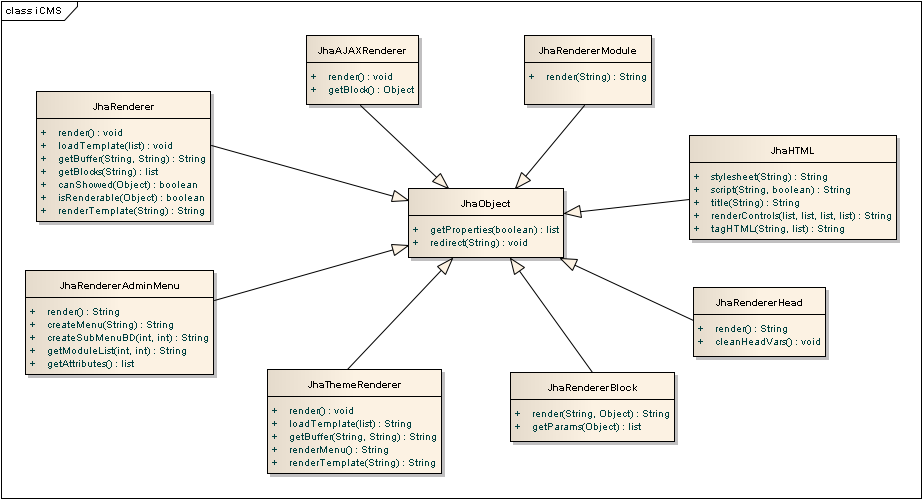
\includegraphics[scale=.45, keepaspectratio=true]{imagenes/10_imagen.png}
\caption{Modelo de clases: Renderizadores. [Elaboraci\'on propia].}
\end{figure}

A continuaci\'on vemos en detalle cada uno de los renderizadores.\\

El renderizador \textit{JhaRenderer} hereda de la clase \textit{JhaObject}, este se encarga de renderizar la plantilla entera, es decir que de alguna manera este hace uso de los dem\'as renderizadores.\\
Los siguientes m\'etodos son parte de este renderizador:
\begin{description}
\item[render] B\'asicamente este m\'etodo es el punto de partida para la renderizaci\'on.
\item[loadTemplate] Retorna la plantilla como si fuera una cadena para hacerla m\'as manejablea nivel de c\'odigo.
\item[renderTemplate] Recibe como parametro el resultado de ``loadTemplate'', en base a este parametro agrega contenidos que son los resultados de los otros renderizadores.
\item[getBuffer] Este m\'etodo act\'ua como discriminador, dependiendo del tipo de contenido que debe mostrarse llama a uno u otro renderizador. En el caso de los bloques hace una comprobaci\'on adicional que le permite saber si un bloque se debe mostrar o no a trav\'es de los m\'etodos ``canShowed'' e ``isRenderable''.
\item[getBlocks] Es un m\'etodo auxiliar para ``getBuffer''.
\end{description}

\begin{lstlisting}[label=jha_renderer,caption=Renderizador JhaRenderer.]
<?php
...

class JhaRenderer extends JhaObject {
	public function render(){
		$db = &JhaFactory::getDBO();
        $db->setQuery('SELECT * FROM #__plantilla WHERE predeterminado = 1');
        $row = $db->loadObject();
        
		$template = $this->loadTemplate($row);
		echo $this->renderTemplate(str_replace('<jhadoc:include type="maincontent" />', $row->html, $template));
	}
	 
	protected function loadTemplate($row){
        $template = '';
		ob_start();
        require_once JHA_THEMES_PATH.DS.($row ? $row->nombre : 'default').DS.'index.php';
        $template = ob_get_contents();
        ob_end_clean();
        return $template;
	}
	
	protected function getBuffer($type = null, $region = null){
		$content = '';
		if($type == null){
		    return;
		}
		$renderer = &JhaFactory::getRenderer($type);
		if($type == 'module'){
			$GLOBALS['JHA_MODULE_PATH'] = JHA_BASE_PATH.DS.'modules'.DS.JhaRequest::getVar('elem','mod_content').DS;
			$path = $GLOBALS['JHA_MODULE_PATH'].substr(JhaRequest::getVar('elem', 'mod_content'),4).'.php';
			$content = $renderer->render($path).$content;
		}
		elseif ($type == 'block' && $region != null){
			$blocks = $this->getBlocks($region);
			if($blocks) {
				if(JhaUtility::userCanEdit()){
				    $content .= '<div class="jhablock"><div class="jhablock-header">Region: ' . ucfirst($region) . '</div>';
				    $script = '';
		        }
				foreach($blocks as $block) {
					if($this->isRenderable($block) && $this->canShowed($block)){
						$GLOBALS['JHA_BLOCK_PATH'] = JHA_BASE_PATH.DS.'blocks'.DS.$block->renderizador.DS;
						$path = $GLOBALS['JHA_BLOCK_PATH'] . substr($block->renderizador,6) . '.php';
						$content .= $renderer->render($path, $block);
						if(JhaUtility::userCanEdit()){
							$script .= "dragBlock.addTarget(Jha.dom.$('block" . $block->id . "'));\n";
						}
					}
				}
				if(JhaUtility::userCanEdit()){
					//aumentar final de bloque y tb. la opcion de Add more blocks
					//la opcion se abrira en un iframe.
					$content .= JhaHTML::script($script, false);
					//agregar el enlace para agregar nuevos bloques.
					$content .= (JhaUtility::userCanAdministrate() ? '<div><a href="index.php?elem=mod_base&controller=block&task=newblock&region=' . $region . '"><img src="images/new.jpg" title="Agregar nuevo bloque" /></a></div>' : '');
					$content .= '</div>';
				}
			}
			else {
				if(JhaUtility::userCanEdit()){
					$content .= '<div class="jhablock"><div class="jhablock-header">Region: ' . ucfirst($region) . '</div>' . (JhaUtility::userCanAdministrate() ? '<div><a href="index.php?elem=mod_base&controller=block&task=newblock&region=' . $region . '"><img src="images/new.jpg" title="Agregar nuevo bloque" /></a></div>' : '') . '</div>';
				}
			}
		}
		elseif ($type == 'head' || ($type == 'admin-menu' && JhaUtility::userCanAdministrate())){
            $content = $renderer->render().$content;
        }
		return $content;
	}
	
	protected function getBlocks($region){
		$db = &JhaFactory::getDBO();
        $db->setQuery("SELECT * FROM #__bloque WHERE region = '" . $region . "' ORDER BY orden ASC");
        return $db->loadObjectList();
	}
	
	protected function canShowed($block){
		if(JhaUtility::userCanEdit()){
			return true;
		}
		return 0 == intval($block->needlogin);
	}
	
	protected function isRenderable($block){
		$db = &JhaFactory::getDBO();
        $itemid = JhaRequest::getVar('itemid',0);
        if($itemid == 0){
            $db->setQuery('SELECT * FROM #__menuitem WHERE home = 1');
            $row = $db->loadObject();
            $itemid = $row->id;
        }
        $db->setQuery("SELECT * FROM #__menubloque WHERE (idmenu = '" . $itemid . "' OR idmenu = '0' ) AND idbloque = '" . $block->id . "'");
        $row = $db->loadObject();
        if($row)
            return true;
        return false;
	}
	
	protected function renderTemplate($template) {
        if(JhaUtility::userCanEdit()){
        	$GLOBALS['JHA_HEAD_VARS'][] = JhaHTML::script("dragBlock = new Jha.drag();\ndragBlock.setType('block');\ndragBlock.ajaxPost = function (objajax, idSource, idTarget, isBeforeTarget) { objajax.json = true; res = { elem : 'mod_base', controller : 'block', src : idSource, trg : idTarget, json : objajax.json, before : isBeforeTarget, task : 'reorder'}; return res; };", false);
        }
		$replace = array();
        $matches = array();
        if(preg_match_all('#<jhadoc:include\ type="([^"]+)" (.*)\/>#iU', $template, $matches)) {
            $matches[0] = array_reverse($matches[0]);
            $matches[1] = array_reverse($matches[1]);
            $matches[2] = array_reverse($matches[2]);
            $count = count($matches[1]);
            for($i = 0; $i < $count; $i++) {
                $attribs = JhaUtility::parseAttributes( $matches[2][$i] );
                $replace[$i] = $this->getBuffer($matches[1][$i], (isset($attribs['region']) ? $attribs['region'] : null));
            }
            $template = str_replace($matches[0], $replace, $template);
        }
        return $template;
	} 
}
?>
\end{lstlisting}


El renderizador \textit{JhaRendererModule} tambi\'en hereda de la clase \textit{JhaObject}, este se encarga de renderizar los m\'odulos unicamente.\\
Este renderizador solamente cuenta con el m\'etodo render ya que no necesita hacer ning'un tipo de comprobaci\'on, de esto se encargan los propios m\'odulos.

\begin{lstlisting}[label=jha_renderer_module,caption=Renderizador de modulos.]
<?php
...

class JhaRendererModule extends JhaObject {
    public function render($path){
        $content = '';
        if(file_exists( $path )){
            ob_start();
            require $path;
            $content = ob_get_contents();
            ob_end_clean();
        }
        return $content;
    }
}
?>
\end{lstlisting}


El renderizador \textit{JhaRendererBlock} al igual que los anteriores, tambi\'en hereda de la clase \textit{JhaObject}, este se encarga de renderizar unicamente los bloques, algo que cabe destacar es que cada bloque tienen un conjunto de configuraciones para lo cual cuenta con un m\'etdo auxiliar para este menester.\\
A continuaci\'on vemos una descripci\'on de los m\'etodos que son parte de este renderizador:
\begin{description}
\item[render] En escencia se encarga de devolver el resultado de renderizar alg\'un bloque.
\item[getParams] Retorna los parametros para el bloque, esta informaci\'on se la obtiene de la base de datos juntamente con el contenido del bloque.
\end{description}

\begin{lstlisting}[label=jha_renderer_block,caption=Renderizador de bloques.]
<?php
...

class JhaRendererBlock extends JhaObject {
	public function render($path, $block){
		$content = '';
		$params = $this->getParams($block);
	    if(file_exists( $path )){
            ob_start();
            require $path;
            if(JhaUtility::userCanEdit()){
                $content .= '<div class="block blockelement' . $params['suffix'] . '" id="block' . $block->id . '"><div class="block-header"><div align="left" style="float:left;"><a href="index.php?elem=mod_base&controller=block&task=editblock&id=' . $block->id . '" title="Editar"><img src="images/edit.jpg" /></a></div><div align="left" onmousedown="javascript:dragBlock.onDragStart(event, Jha.dom.$(\'block' . $block->id . '\'));" style="line-height: 2;">' . $block->titulo . '</div></div>' . ob_get_contents() . '</div>';
            }
            else {
                $content = '<div class="blockelement' . $params['suffix'] . '">' . ob_get_contents() . '</div>';
            }
            ob_end_clean();
        }
        return $content;
	}
	
	public function getParams($block){
		$params = split("\n",$block->params);
		$res = array();
		foreach ($params as $param){
			$parts = split('=', $param);
			$res[$parts[0]] = $parts[1];
		}
		return $res;
	}
}
?>
\end{lstlisting}


El renderizador \textit{JhaRendererHead} se encarga de renderizar unicamente elementos que van en el tag HTML ``head''.\\
A continuaci\'on vemos una descripci\'on de los m\'etodos que son parte de este renderizador:
\begin{description}
\item[render] Renderiza los las hojas de estilo (CSS) y los scripts (JS) dependiendo del tipo de sesi\'on.
\item[cleanHeadVars] Esto limpia los elementos duplicados, adem\'as crea un orden entre los elementos que son parte del tag ``tag''.
\end{description}

\begin{lstlisting}[label=jha_renderer_head,caption=Renderizador para el tag HTML `head'.]
<?php
...

class JhaRendererHead extends JhaObject {
  public function render(){
    $content = '';
    $GLOBALS['JHA_HEAD_VARS'] = (isset($GLOBALS['JHA_HEAD_VARS'][0]) ? $GLOBALS['JHA_HEAD_VARS'] : array());
    if(JhaUtility::userCanEdit()){
    	$GLOBALS['JHA_HEAD_VARS'] = array_reverse($GLOBALS['JHA_HEAD_VARS']);
    	$GLOBALS['JHA_HEAD_VARS'][] = JhaHTML::script('libraries/jhaley/js/menu.js');
    	$GLOBALS['JHA_HEAD_VARS'][] = JhaHTML::script('libraries/jhaley/js/popup.js');
    	$GLOBALS['JHA_HEAD_VARS'][] = JhaHTML::script('libraries/jhaley/js/pmenu.js');
    	$GLOBALS['JHA_HEAD_VARS'][] = JhaHTML::script('libraries/jhaley/js/effect.js');
    	$GLOBALS['JHA_HEAD_VARS'][] = JhaHTML::script('libraries/jhaley/js/drag.js');
    	$GLOBALS['JHA_HEAD_VARS'][] = JhaHTML::script('libraries/jhaley/js/ajax.js');
      $GLOBALS['JHA_HEAD_VARS'][] = JhaHTML::script('libraries/jhaley/js/jha.js');
      $GLOBALS['JHA_HEAD_VARS'][] = JhaHTML::stylesheet('libraries/jhaley/css/menu.css');
      $GLOBALS['JHA_HEAD_VARS'][] = JhaHTML::stylesheet('libraries/jhaley/css/base.css');
      $GLOBALS['JHA_HEAD_VARS'] = array_reverse($GLOBALS['JHA_HEAD_VARS']);
    }
    else{
    	$GLOBALS['JHA_HEAD_VARS'] = array_reverse($GLOBALS['JHA_HEAD_VARS']);
    	$GLOBALS['JHA_HEAD_VARS'][] = JhaHTML::script('libraries/jhaley/js/effect.js');
      $GLOBALS['JHA_HEAD_VARS'][] = JhaHTML::script('libraries/jhaley/js/jha.js');
      $GLOBALS['JHA_HEAD_VARS'] = array_reverse($GLOBALS['JHA_HEAD_VARS']);
    }
    if(isset($GLOBALS['JHA_HEAD_VARS']) && count($GLOBALS['JHA_HEAD_VARS']) > 0){
    	$this->cleanHeadVars();
        $content .= implode('',$GLOBALS['JHA_HEAD_VARS']);
    }
    return $content;
  }
  
  protected function cleanHeadVars(){
  	$array = array();
  	foreach ($GLOBALS['JHA_HEAD_VARS'] as $headVar){
  		if (JhaUtility::inArray($headVar, $array) == -1) {
  			$array[] = $headVar;
  		}
  	}
  	$GLOBALS['JHA_HEAD_VARS'] = $array;
  }
}
?>
\end{lstlisting}


El renderizador \textit{JhaAJAXRenderer} se encarga de renderizar unicamente bloques y/o m\'odulos. Este renderizador no sigue el flujo normal que es pasar por la clase \textit{JhaRenderer}, sino que como su nombre indica esta dise\~nado para las peticiones as\'incronas.\\
Los m\'etodos que son parte de este renderizador son:
\begin{description}
\item[render] Renderiza bloques y m\'odulos dependiendo de la petici\'on AJAX.
\item[getBlock] Recupera los datos del bloque, si es que la petici\'on AJAX est\'a relacionada con los bloques.
\end{description}

\begin{lstlisting}[label=jha_renderer_ajax,caption=Renderizador las llamadas as\'incronas.]
<?php
...

class JhaAJAXRenderer extends JhaObject {
    public function render(){
        $content = '';
        $elem = JhaRequest::getVar('elem');
        if(substr($elem, 0, 3) == 'mod'){
        	$renderer = &JhaFactory::getRenderer('module');
        	$GLOBALS['JHA_MODULE_PATH'] = JHA_BASE_PATH.DS.'modules'.DS.$elem.DS;
            $path = $GLOBALS['JHA_MODULE_PATH'].substr($elem, 4).'.php';
            $content = $renderer->render($path).$content;
        }
        else {
        	$block = $this->getBlock();
        	$renderer = &JhaFactory::getRenderer('block');
        	$GLOBALS['JHA_BLOCK_PATH'] = JHA_BASE_PATH.DS.'blocks'.DS.$block->renderizador.DS;
            $path = $GLOBALS['JHA_BLOCK_PATH'] . substr($block->renderizador,6) . '.php';
            $content = $renderer->render($path, $block);
        }
        echo $content;
    }
    
    protected function getBlock(){
    	$db = &JhaFactory::getDBO();
        $db->setQuery("SELECT * FROM #__bloque WHERE id = '" . JhaRequest::getVar('id') . "'");
        return $db->loadObject();
    }
}
?>
\end{lstlisting}


El renderizador \textit{JhaRendererAdminMenu} al igual que los anteriores, tambi\'en hereda de la clase \textit{JhaObject}, este renderizador est\'a destinado unicamente a renderizar el menu de administraci\'on.\\
Los m\'etodos que son parte de este renderizador son:
\begin{description}
\item[render] Renderiza los menus y sub menus de administraci\'on, el resto de m\'etodos son auxiliares para renderizar fragmentos del menu: \textit{createMenu}, \textit{createSubMenuBD}, \textit{getModuleList} y \textit{getAttributes}.
\end{description}

\begin{lstlisting}[label=jha_renderer_admin_menu,caption=Renderizador para el men\'u de administraci\'on.]
<?php
...

class JhaRendererAdminMenu extends JhaObject {
    public function render(){
    	$content = '';
        $user = (isset($_SESSION['USER']) ? $_SESSION['USER'] : NULL);
        $canEdit = $user->rol == 'Super Administrador' || $user->rol == 'Editor';
        if($canEdit){
        	$xml = simplexml_load_file(JHA_LIBRARIES_PATH.DS.'jhaley'.DS.'xml'.DS.'adminmenu.xml');
        	$content .= '<div id="jha-admin-menu"><div style="width: 950px; margin: 0pt auto; height: 25px; background-color: black;">' . $this->createMenu($xml) . '</div></div><br />';
        	$GLOBALS['JHA_HEAD_VARS'][] = JhaHTML::script('document.menu = null;
        	window.onload = function(){
        	    element = Jha.dom.$(\'jhamenu\');
        	    var menu = new Jha.menu(element);
        	    document.menu = menu;
   	        };', false);
        }
        return $content;
    }
    
    protected function createMenu($xml){
    	$content = '<ul' . $this->getAttributes($xml->attributes()) . '>';
   		foreach ($xml->elements->element as $element) {
   			$att = $element->attributes();
   			$content .= '<li><a' . $this->getAttributes($att) . '>' . $element->text . '</a>';
   			if(!isset($element->elements) && $att['type'] == 'bd'){
			    $content .= $this->createSubMenuBD(0);
   			}
   			elseif(isset($element->elements)){
   				$content .= $this->createMenu($element);
   			}
   			$content .= '</li>';
   		}
    	return $content . '</ul>';
    }
    
    protected function createSubMenuBD($level, $id = NULL){
    	$content = '';
    	$links = $this->getModuleList($level, $id);
    	if(count($links) > 0){
    		$content .= '<ul>';
	    	foreach ($links as $link) {
	    		$href = ($link->link != '' ? ' href="' . $link->link . '&itemid=' . $_SESSION["itemid"] . '"' : '');
	    		$content .= '<li><a' . $href . '>' . $link->nombre . '</a>';
	    		$content .= $this->createSubMenuBD($level + 1, $link->id) . '</li>';
	    	}
	    	$content .= '</ul>';
    	}
    	return $content;
    }
    
    protected function getModuleList($level, $id = NULL){
    	$db = &JhaFactory::getDBO();
    	$db->setQuery('SELECT * FROM #__modules WHERE parent = ' . ($level == 0 ? '0' : $id));
        return $db->loadObjectList();
    }
    
    protected function getAttributes($attributes){
    	$attr = '';
    	if(count($attributes) > 0){
    		foreach ($attributes as $index => $value){
    			if($index == 'href'){
    				$attr .= ' ' . $index . '="' . $value . '&itemid=' . $_SESSION["itemid"] . '"';
    			}
    			elseif($index != 'type'){
    			    $attr .= ' ' . $index . '="' . $value . '"';
    			}
    		}
    	}
    	return $attr;
    }
}
?>
\end{lstlisting}


El renderizador \textit{JhaThemeRenderer} tambi\'en hereda de la clase \textit{JhaObject}, este renderizador est\'a destinado unicamente a renderizar la plantilla en modo de personalizaci\'on, esto significa que podremos personalizarla desde la interfaz gr\'afica.\\
Los m\'etodos que son parte de este renderizador son:
\begin{description}
\item[render] Renderiza la plantilla de forma muy similar a \textit{JhaRenderer} con la diferencia de que no renderiza el contenido sino que inserta en su lugar elementos para su manipulaci\'on desde la interfaz gr\'afica, es decir para personalizar la plantilla.
\end{description}

\begin{lstlisting}[label=jha_renderer_head,caption=Renderizador para el tag HTML `head'.]
<?php
...

class JhaThemeRenderer extends JhaObject {
	public function render(){
		$db = &JhaFactory::getDBO();
    $db->setQuery('SELECT * FROM #__plantilla WHERE predeterminado = 1');
    $row = $db->loadObject();
        
		$template = $this->loadTemplate($row);
		$_SESSION['themeHTML'] = isset($_SESSION['themeHTML']) ? $_SESSION['themeHTML'] : $row->html;
		$_SESSION['themeXML'] = isset($_SESSION['themeXML']) ? $_SESSION['themeXML'] : $row->xml;
		echo $this->renderTemplate($template);
	}
	 
	protected function loadTemplate($row){
    $template = '';
		ob_start();
    require_once JHA_THEMES_PATH.DS.($row ? $row->nombre : 'default').DS.'index.php';
    $template = ob_get_contents();
    ob_end_clean();
    return $template;
	}
	
	protected function getBuffer($type = null, $region = null){
		$content = '';
		if($type == null){
	    return;
		}
		$renderer = &JhaFactory::getRenderer($type == 'maincontent' ? 'module' : $type);
		if($type == 'maincontent') {
			$GLOBALS['JHA_MODULE_PATH'] = JHA_BASE_PATH.DS.'modules'.DS.JhaRequest::getVar('elem','mod_content').DS;
			$path = $GLOBALS['JHA_MODULE_PATH'].substr(JhaRequest::getVar('elem', 'mod_content'),4).'.php';
			$content = $renderer->render($path).$content;
		}
		elseif ($type == 'head'){
      $content = $renderer->render().$content;
    }
    elseif ($type == 'admin-menu'){
    	$content = $this->renderMenu().$content;
    }
		return $content;
	}
	
	private function renderMenu(){
		$content = '';
		if(JhaUtility::userCanEdit()) {
    	$content .= '<div id="jha-admin-menu"><div style="width: 950px; margin: 0pt auto; height: 25px; background-color: black;"><ul id="jhamenu"><li><a href="index.php?elem=mod_base&controller=theme&task=savePersonalizedChanges">Guardar Cambios</a></li><li><a href="index.php?elem=mod_base&controller=theme&task=cancelPersonalizedChanges">Cancelar</a></li></ul></div></div><br />';
    	$GLOBALS['JHA_HEAD_VARS'][] = JhaHTML::script('document.menu = null;
    	window.onload = function(){
  	    element = Jha.dom.$(\'jhamenu\');
  	    var menu = new Jha.menu(element);
  	    document.menu = menu;
      };', false);
    }
    return $content;
	}
	
	protected function renderTemplate($template) {
		$replace = array();
    $matches = array();
    if(preg_match_all('#<jhadoc:include\ type="([^"]+)" (.*)\/>#iU', $template, $matches)) {
      $matches[0] = array_reverse($matches[0]);
      $matches[1] = array_reverse($matches[1]);
      $count = count($matches[1]);
      for($i = 0; $i < $count; $i++) {
        $replace[$i] = $this->getBuffer($matches[1][$i]);
      }
      $template = str_replace($matches[0], $replace, $template);
    }
    return $template;
	} 
}
?>
\end{lstlisting}


La clase \textit{JhaHTML} no es precisamente un renderizador de contenido especializado como el de los m\'odulos o bloques, pero en su lugar es capaz de generar contenido HTML simple como tags `link', `script' y `title'.\\
Los m\'etodos que son parte de este renderizador son:
\begin{description}
\item[stylesheet] Renderiza un tag `link' con alguna hoja de estilos.
\item[script] Renderiza un tag `script' con alg\'un contenido javascript ya sea contenido en linea o desde un archivo.
\item[title] Renderiza un tag `title' con el titulo de la p\'agina.
\item[tagHTML] Renderiza un tag HTML arbitrario.
\item[renderControls] Renderiza el conjunto de controles de administraci\'on de contenidos, es decir los controles de Nuevo, Editar, Eliminar, Guardar, Cancelar. En el panel de administraci\'on estos controles son muy comunes, as\'i que este m\'etodo facilita mucho su creaci\'on
\end{description}

\begin{lstlisting}[label=jha_renderer_head,caption=Renderizador para el tag HTML `head'.]
<?php
...

class JhaHTML extends JhaObject {
    
  public static function stylesheet($url){
  	jhaimport('jhaley.web.tags');
    $taghtml = new Tag ('link');
    $taghtml->setAttribute('type', 'text/css');
    $taghtml->setAttribute('rel', 'stylesheet');
    $taghtml->setAttribute('href', $url);
    return $taghtml->html ();
  }
    
  public static function script($src, $isUrl = true){
  	jhaimport('jhaley.web.jstag');
    $tagjs = new JSTag ();
    if($isUrl){
      $tagjs->setAttribute('type', 'text/javascript');
      $tagjs->setAttribute('src', $src);
    }
    else{
      $tagjs->add($src);
    }
    return $tagjs->html ();
  }
  
  public function title($title = ''){
  	jhaimport('jhaley.web.tags');
  	$taghtml = new Tag ('title', $title);
  	return $taghtml->html ();
  }
  
  //array-> titulos, tasks, linktype**, icons.  
  // ** -> Para la validacion de los checkboxes.
  public function renderControls($titles, $tasks, $linktypes, $icons){
  	if(count($titles) <= 0 && count($tasks) <= 0 && count($linktypes) <= 0) return '';
  	jhaimport('jhaley.web.tags');
  	$tagtable = new Tag ('table');
  	$tagtable -> add( $tagtr = new Tag('tr') );
    for($i = 0; $i < count($titles); $i++){
    	$mustValidate = $linktypes[$i] == 'edit' || $linktypes[$i] == 'delete' || $linktypes[$i] == 'save';
    	$onclick = '';
    	if($mustValidate) {
    		$condicion = ($linktypes[$i] == 'edit' || $linktypes[$i] == 'delete' ? 'Jha.html.checkbox.validate()' : 'validateForm()');
    		$onclick = 'if(' . $condicion . '){Jha.dom.$(\'task\').value = \'' . $tasks[$i] . '\'; document.forms.adminForm.submit();}';
    	}
    	else {
    		$onclick = 'Jha.dom.$(\'task\').value = \'' . $tasks[$i] . '\'; document.forms.adminForm.submit();';
    	}
      if($icons != null && $icons[$i] != null){
      	$tagicon = new Tag('img');
      	$tagicon->setAttribute('src', $icons[$i]);
      	$tagicon->setAttribute('title', $titles[$i]);
      }
      else{
      	$tagicon = new Tag('span');
      	$tagicon -> setAttribute('class', 'icon-' . $linktypes[$i]);
      	$tagicon -> setAttribute('title', $titles[$i]);
      }
      $tagtr -> add( $tagtd = new Tag('td') );
      $tagtd -> add( $taga = new Tag('a') );
      $taga -> setAttribute('href', 'javascript:;');
      $taga -> setAttribute('onclick', 'javascript:' . $onclick);
      $taga -> add( $tagicon );
      $taga -> add( $titles[$i] );
    }
    return $tagtable->html ();
  }
  
  public function tagHTML($tag = 'p', $extras = array()) {
  	jhaimport('jhaley.web.tags');
    $taginput = new Tag ('input');
    foreach ($extras as $index => $value) {
    	$taginput->setAttribute($index, $value);
    }
    return $taginput->html ();
  }
}
?>
\end{lstlisting}


\subsection{Modelo de Base de Datos}
El modelo de base de datos o modelo Entidad-Relaci\'on, contiene tablas que son propias del motor de renderizado de plantillas, tambi\'en est\'an presentes algunas tablas que son parte de las extensiones (contenido, menu). Escencialmente son extensiones, pero a la vez son una parte fundamental del \textit{i}CMS.

\begin{figure}[h]
\centering
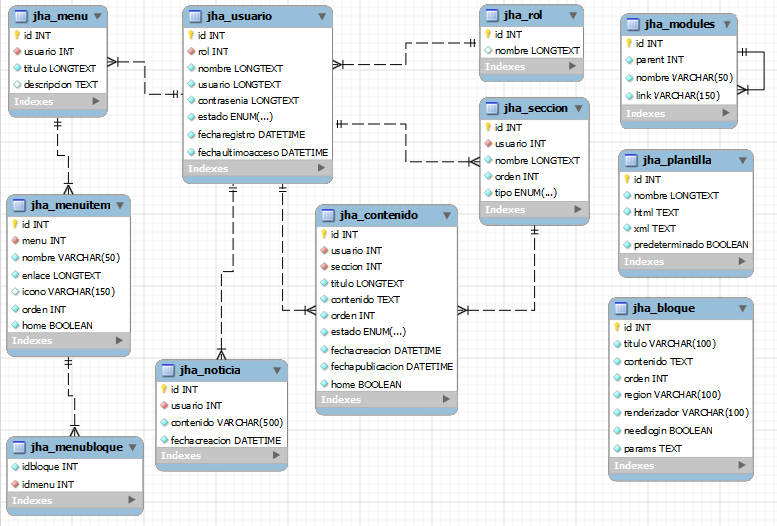
\includegraphics[scale=.6, keepaspectratio=true]{imagenes/12_imagen.png}
\caption{Modelo de Base de Datos. [Elaboraci\'on propia].}
\end{figure}

\section{M\'odulos, Bloques y Temas}
Se presenta una descripci\'on de las distintas extensiones que forman parte del \textit{i}CMS, de forma general las extensiones estan compuestas por m\'odulos, bloques y temas, veremos en detalle la estructura tanto a nivel de clases como a nivel de directorios. Al estar trabajando con un lenguaje de PostScripting como PHP, muchos de los archivos no aparecen en el modelo de clases, justamente por que no son clases como tal.

\subsection{Estructura de los m\'odulos}
Todos los m\'odulos siguen el patr\'on Modelo-Vista-Controlador, adem\'as maneja un archivo el cual se convierte en punto de entrada para el modulo, la finalidad de este archivo es para ejecutar el m\'etodo correcto del controlador dependiendo de la acci\'on requerida a trav\'es de los parametros del REQUEST.

\subsection{Estructura de los bloques}
Los bloques se registran en la base de datos, tienen en com\'un un campo llamado \textit{params} el cual sirve para establecer los parametros que definen como se debe mostrar\'a el contenido del bloque.\\
Por otro lado varios de los bloques, tienen un archivo denominado \textit{helper}, que se encarga de proveer funciones de acceso a datos y utilidades.
Todos los renderizadores de bloques llevan un archivo \textit{param.php}, el cual sirve para definir los parametros de cada bloque.

\subsection{Relaci\'on entre m\'odulos y bloques}
Los bloques y m\'odulos no guardan relaci\'on a nivel de c\'odigo, cada uno tiene una finalidad espec\'ifica.\\
Los m\'odulos procesan las interacciones del usuario con el sistema, es decir, que cada solicitud que el usuario hace al sistema es procesada a trav\'es de alg\'un m\'odulo. Como resultado de este procesamiento, se genera contenido HTML, el cual se ubica en una regi\'on particular de la plantilla a trav\'es de los renderizadores.\\
Los bloques por otro lado, solo se encargan de mostrar contenido, y lo hacen en regiones distintas a las del m\'odulo.

\subsection{M\'odulos}
A continuaci\'on vemos los distintos m\'odulos que forman parte de \textit{i}CMS.

\subsubsection{M\'odulo Base}
El m\'odulo base contiene funciones b\'asicas para el funcionamiento del CMS, tales como: la personalizaci\'on de la plantilla, agregado de nuevas plantillas, gestionado de bloques de contenido, configurado del CMS, entre otras.

\begin{figure}[h]
\centering
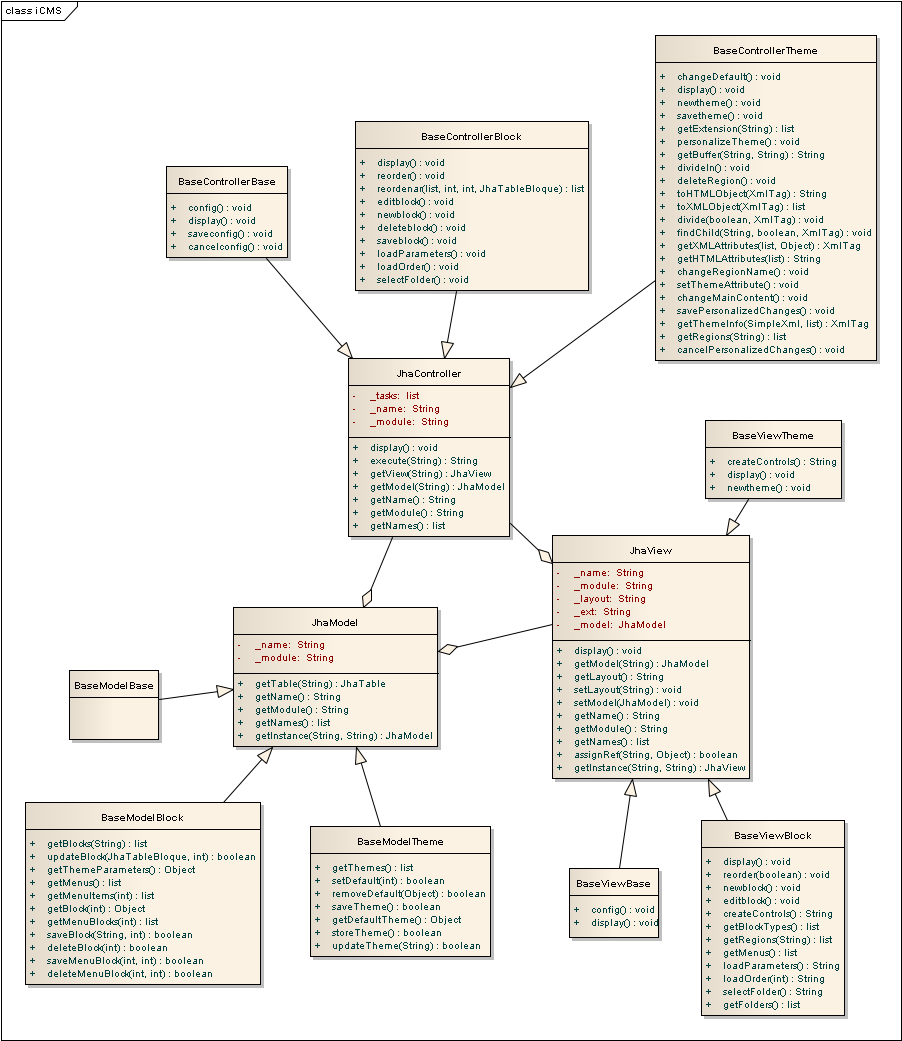
\includegraphics[scale=.35, keepaspectratio=true]{imagenes/13_imagen.png}
\caption{Modelo de clase: M\'odulo Base. [Elaboraci\'on propia].}
\end{figure}

\subsubsection{Configurado del CMS}
La configuraci\'on del CMS se hace a trav\'es del archivo \textit{JhaConfiguration}, gestiona los datos del servidor de base de datos as\'i como el prefijo de las tablas, tambi\'en se puede gestionar la vigencia de las noticias y tambi\'en los meta-datos para lo que se conoce como \textit{alta en buscadores}.

\subsubsection{Gesti\'on de plantillas}
La gesti\'on de plantillas comprende dos elementos importantes.\\
El primero de estos elementos, permite agregar nuevas plantillas e intercambiar la apariencia de la p\'agina a trav\'es de las plantillas.\\
Las plantillas que se suben al servidor deben tener una estructura concreta. Se deben tener m\'inimamente los siguientes archivos en un compreso ya sea tar.gz, tar.bz:
\begin{itemize}
\item index.php
\item info.xml
\item install.sql
\end{itemize}
\ldots\ Adicionalmente se pueden tener un directorio para im\'agenes y otro directorio para los css.\\
El segundo elemento permite personalizar la plantilla que se designa por defecto para mostrarse en el sitio. Para este efecto el m\'odulo provee mecanismos para ver las regiones definidas en la plantilla, asimismo tiene mecanismos para dividir las regiones ya sea en columnas o filas. Tambi\'en las regiones pueden moverse para reacomodar las regiones.\\
Este motor de gesti\'on de las plantillas provee una gama de opciones para que el usuario pueda personalizar a\'un m\'as su plantilla.

\subsubsection{Gesti\'on de bloques}
Los bloques son los contenidos secundarios, todos los bloques trabajan de forma muy similar, todas ellas tienen un renderizador espec\'ifico, en s\'intesis cada bloque tiene su propio renderizador.\\
A trav\'es de este gestor de bloques se definen elementos como la regi\'on donde se mostrar\'a el bloque, el orden entre bloques, y la relaci\'on entre los bloques y los men\'us, todo esto a nivel de administraci\'on avanzada del \textit{i}CMS, cuando hablamos de una administraci\'on est\'andar, hacemos referencia a los cambios que se pueden hacer directamente manipulando el contenido sobre la plantilla, o como decimos vulgarmente, ``En caliente''.

\subsubsection{M\'odulo Content}
El m\'odulo de contenido contiene funciones para el gestionamiento de las publicaciones del CMS, tales como: la gesti\'on de art\'iculos, gesti\'on de secciones y gesti\'on de noticias.

\begin{figure}[h]
\centering
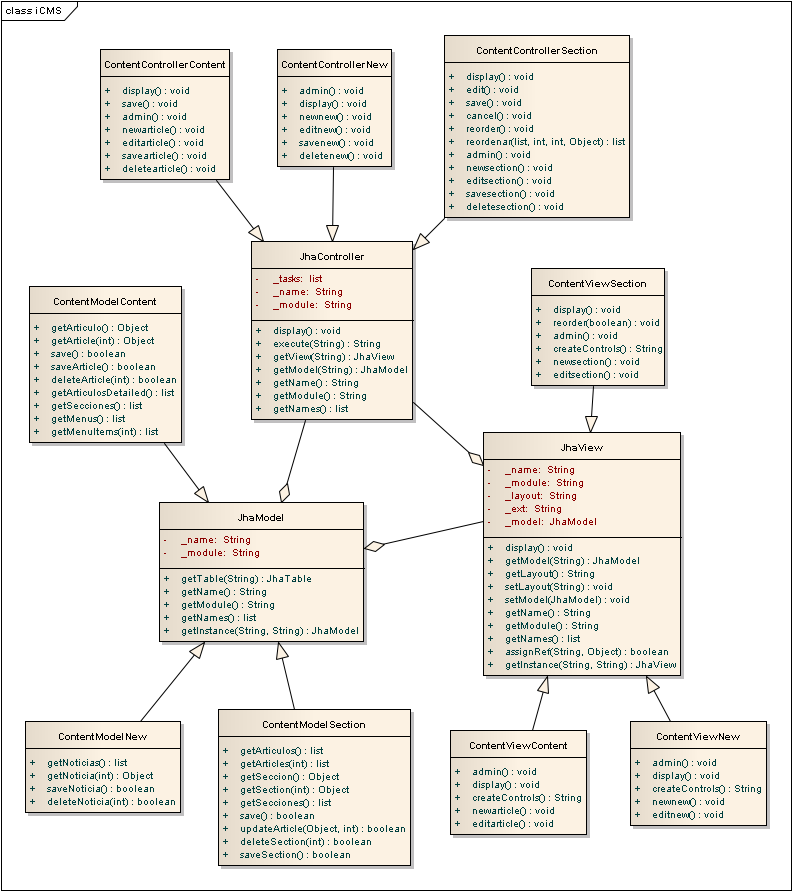
\includegraphics[scale=.4, keepaspectratio=true]{imagenes/14_imagen.png}
\caption{Modelo de clase: M\'odulo Content. [Elaboraci\'on propia].}
\end{figure}

\subsubsection{Gesti\'on de art\'iculos}
A trav\'es de este medio se pueden crear, editar, eliminar y listar los art\'iculos, los art\'iculos pertenecen a una secci\'on, adem\'as cada art\'iculo puede estar o no relacionado a un item de men\'u. Tambi\'en se cuenta con el editor WYSIWG para agregar el contenido de los art\'iculos.

\subsubsection{Gesti\'on de secciones}
Las secciones muestran un conjunto de art\'iculos al mismo tiempo, por el momento solo maneja una vista est\'andar de dos columnas, donde en la primera se muestra el art\'iculo mas reciente, y en la segunda se muestran los art\'iculos anteriores.\\
Las secciones al igual que los art\'iculos, tambi\'en estan relacionados a un enlace de men\'u.

\subsubsection{Gesti\'on de noticias}
Las noticias solo son p\'arrafos muy breves, avisos muy cortos que se sirven del bloque de noticias para mostrarse.\\
Al igual que la gesti\'on de secciones y art\'iculos se pueden crear, editar, listar y eliminar las noticias.

\newpage
\subsubsection{M\'odulo Men\'u}
El m\'odulo de men\'us contiene funciones para el gestionamiento de los men\'us del CMS.

\begin{figure}[h]
\centering
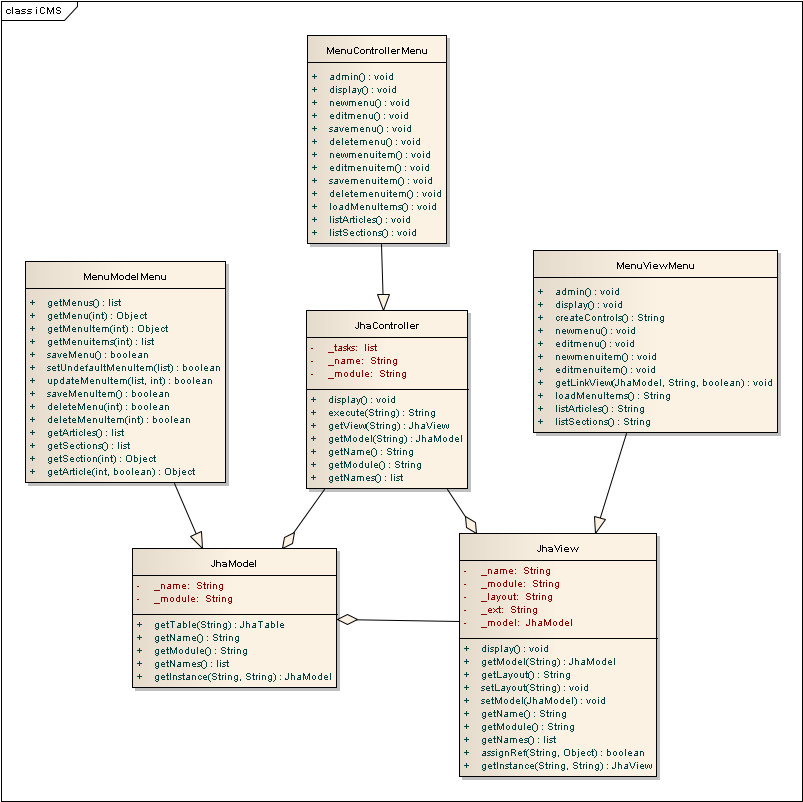
\includegraphics[scale=.4, keepaspectratio=true]{imagenes/15_imagen.png}
\caption{Modelo de clase: M\'odulo Men\'u. [Elaboraci\'on propia].}
\end{figure}

\subsubsection{Gesti\'on de men\'us}
La gesti\'on de men\'us contiene dos elementos: Los men\'us propiamente dichos y los \'items de men\'u.\\
Los men\'us solo agrupan un conjunto de \'items de men\'u.\\
Los \'items de men\'u contiene un enlace a art\'iculos, secciones o a p\'aginas externas al sitio, cada \'item de men\'u tiene un n\'umero de orden con respecto a los otros \'items del men\'u, tambi\'en pueden tener un \'icono asociado.

\subsubsection{M\'odulo User}
El m\'odulo de usuario contiene funciones para el gestionamiento de los usuarios del CMS.

\begin{figure}[h]
\centering
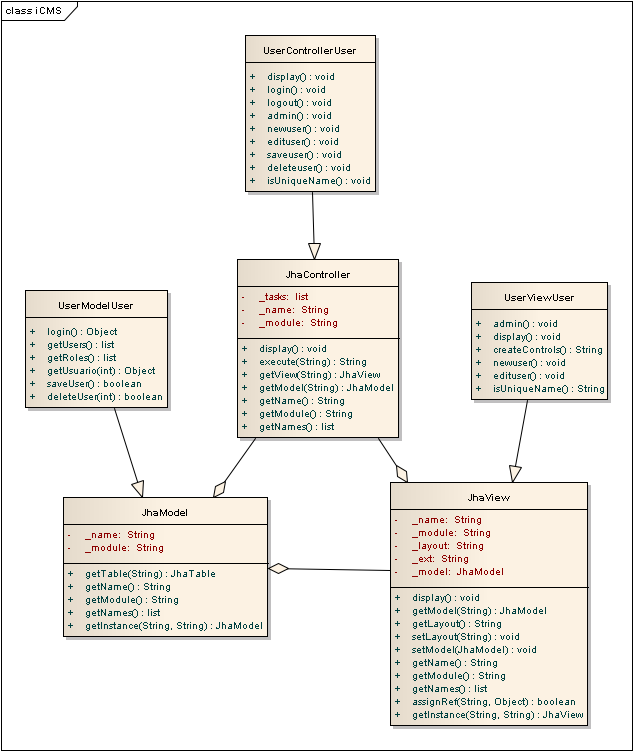
\includegraphics[scale=.4, keepaspectratio=true]{imagenes/16_imagen.png}
\caption{Modelo de clase: M\'odulo User. [Elaboraci\'on propia].}
\end{figure}

\subsubsection{Gesti\'on de usuarios}
A trav\'es de este gestor se pueden crear, modificar, eliminar y listar los usuarios registrados, los usuarios tienen roles definidos (Super Administrador, Editor) y el usuario visitante que no necesita registrarse. Dado que este CMS es un prototipo, no se contempla muchos de los datos de los usuarios.

\subsection{Bloques}
Como ya vimos en el cap\'itulo VI los bloques tienen renderizadores espec\'ificos, en este cap\'itulo veremos la especificaci\'on de cada uno de estos renderizadores de bloques.

\subsubsection{Bloque Banner}
Este renderizador sirve para mostrar banners de im\'agenes, estos banners dependiendo de los parametros del bloque pueden estar animados o no, los efectos son por defecto los que estan presentes en la librer\'ia \textit{effect} del \textit{framework jhaley} (sobreponer, entrar/salir vertical, entrar/salir horizontal).

\subsubsection{Bloque Breadcrumb}
El renderizador de la barra de navegaci\'on es bastante \'util, este renderizador crea los enlaces de la barra de navegaci\'on en funci\'on del men\'u, y va creaciendo con los enlaces de los art\'iculos.

\subsubsection{Bloque Custom}
Quiz\'as este renderizador sea el m\'as \'util, dado que la finalidad que tiene es de crear HTML personalizado. El HTML puede ser de cualquier tipo (im\'agenes, flash, etc.). Al momento de crear los bloques con este renderizador tambi\'en se crea el contenido HTML.

\subsubsection{Bloque Login}
Este renderizador tiene la finalidad de crear la ventana de acceso a las cuentas de usuario, el bloque de login trabaja en conjunto con el m\'odulo de usuario para validar los datos del usuario o tambi\'en para cerrar la sesi\'on del usuario

\subsubsection{Bloque Men\'u}
En cap\'itulos anteriores vimos el m\'odulo de men\'u, en el cual se gestiona los men\'us e \'items de men\'u, pues bien, este renderizador muestra los \'items de men\'u ordenados de acuerdo a un n\'umero de orden, cada bloque de men\'u puede acomodarse en men\'us verticales, horizontales, vertical en listas, tambi\'en es posible hacer visibles o no los iconos asociados a los \'items de men\'u.

\subsubsection{Bloque New}
Este renderizador trabaja en conjunto con el m\'odulo de contenido, concretamente con el gestor de noticias, este bloque solo se encarga de mostrar las noticias, las noticias pueden tener efectos animados dado que tambi\'en utilizan los efectos de la librer\'ia \textit{effect} del \textit{framework jhaley}.

\subsection{Temas}
En este cap\'itulo se tiene una descripci\'on de los temas que forman parte del CMS. Los temas o \textit{templates} son simplemente elementos que le dan al CMS la apariencia en funci\'on de los CSS e im\'agenes.\\
Por el momento se tiene dos temas creados especificamente para el CMS:

\begin{itemize}
\item \begin{description}
	\item[Tema Default] Este tema est\'a creado como apariencia por defecto del CMS
\end{description}
\item \begin{description}
	\item[Tema Enikma] Este tema es una alternativa de apariencia para el CMS.
\end{description}
\end{itemize}

\section{Framework Jhaley}
Como todo CMS tiene un conjunto de librer\'ias definidas para su funcionamiento, iCMS no es la excepci\'on, en el presente cap\'itulo se presenta un vistazo general de los elementos del ``Framework Jhaley'' creados para desarrollar este CMS, dise\~nado para hacer de la reutilizaci\'on de c\'odigo algo innato en el desarrollo del CMS y principalmente para el soporte de nuevas extensiones y en los est\'andares necesarios para el CMS.\\
El framework contempla elementos para ciertas acciones concretas como: 
\begin{itemize}
\item Gesti\'on de variables REQUEST.
\item Gesti\'on de archivos compresos (*.tar, *.tgz, *.tbz).
\item Conexiones y manipulaci\'on de datos (Base de Datos).
\item Gesti\'on de archivos y directorios.
\item Renderizadores.
\item Librer\'ias Javascript.
\item Patr\'on MVC
\item Librer\'ias para gesti\'on de elementos web.
\item Gesti\'on de XML.
\item Librer\'ias para editor WYSIWYG (``What You See Is What You Get'').
\end{itemize}
\ldots\ Entre otras.

\subsection{Arquitectura del Framework}
El framework \textit{Jhaley} para el motor de renderizado utiliza un patr\'on arquitect\'onico de Modelo-Vista-Controlador, gracias a este patr\'on todas las extensiones estan obligadas a seguirlo tambi\'en, la principal ventaja de esta ``regla'' es que todas las extensiones estan muy bienestructuradas facilintando el mantenimineto de las mismas.\\

\subsection{Librer\'ia JhaFactory}
La librer\'ia JhaFactory, como su nombre indica sigue el patr\'on de dise\~no ``\textit{Factory}'', el cual se encarga de tener \'unicamente funciones dispuestas para la creaci\'on de instancias de otros objetos. En nuestro caso en concreto se encarga de crear instancias como:
\begin{itemize}
\item \textbf{JhaDBO}, Objeto de Conexion a la base de datos.
\item \textbf{JhaConfiguration}, Objeto de configuraci\'on general del CMS para un sitio en concreto.
\item \textbf{Renderers}, Objetos de Renderizaci\'on (\textsf{JhaRenderer}, \textsf{JhaModuleRenderer}, \textsf{JhaBlockRenderer}, etc).
\item \textbf{JhaEditor}, Instancia del editor WYSIWYG.
\end{itemize}
Tambi\'en cabe destacar que JhaFactory al igual que otras clases es global con respecto del sistema, esto significa que puede ser utilizado desde cualquier punto dentro de la aplicaci\'on.

\subsection{Librer\'ia JhaRequest}
La librer\'ia JhaRequest, es una clase global que provee funciones est\'aticas para la manipulaci\'on principalmente de las variables del HTMLRequest (REQUEST, POST, GET), pero su uso tambi\'en est\'a en las variables SERVER, SESSION.\\
Entre las funciones que cumple est\'a el que tiene la capacidad de filtrar los valores que se obtienen del HTMLRequest, bajo tres criterios bien marcados:
\begin{itemize}
\item \begin{description}
	\item[NOTRIM] Este filtro le permite considerar como v\'alido el valor obtenido no importando si dicho valor lleva espacios al inicio o final.
	\end{description}
\item \begin{description}
	\item[ALLOWRAW] Este filtro le permite considerar como v\'alido el valor obtenido sin ninguna restricci\'on.
	\end{description}
\item \begin{description}
	\item[ALLOWHTML] Este filtro le permite considerar como v\'alido el valor obtenido solo si es HTML.
	\end{description}
\end{itemize}
Tambi\'en tiene una directiva que le permite obtener un conjunto de valores (Lista), siempre y cuando los nombres con los que llegaron dichos valores tienen un prefijo en com\'un.
%%insertar ejemplo en codigo.

\subsection{Librer\'ia de Utilidades (JhaUtility)}
Est\'a librer\'ia ofrece funciones est\'andar de ayuda para realizar distintas tareas tales como: Buscar un elemento en funcion de su id, ver si un elemento pertenece a una lista, remover un elemento de una lista, insertar un elemento en una posici\'on dada de una lista, verificar si los usuarios son Editores o Administradores.

\subsection{Librer\'ia Import}
Est\'a librer\'ia no contiene una clase sino mas bien una funci\'on, cuyo \'unico trabajo es importar las librer\'ias del framework en cualquier parte de la aplicaci\'on. Recibe una cadena con el formato \textsf{'jhaley.mvc.model'}, donde los puntos representan la sucesi\'on de los paquetes, en este caso el paquete \textsf{mvc} est\'a dentro del paquete \textsf{jhaley}, el \'ultimo elemento, vale decir \textsf{model}, es la librer\'ia como tal.\\
Obviamente que para poder acceder al archivo de la librer\'ia de manera interna se construye la ruta absoluta.

\subsection{Librer\'ias del paquete \textsf{base}}
\subsubsection{JhaObject}
Esta librer\'ia provee un objeto base est\'andar con ciertas caracter\'isticas que son comunes a todos las clases del sistema.\\Las propiedades que define son: 
\begin{itemize}
\item \textsf{getProperties(\$isPublic:boolean):array}, cada objeto es capaz de devolver la lista de sus atributos, si \textsf{\$isPublic} es \textsf{true} devuelve solo los atributos p\'ublicos.
\item \textsf{redirect(\$url:String):void}, cada objeto es capaz de redireccionar a una direcci\'on distinta por medio del par\'ametro \textsf{\$url}.
\end{itemize}

\subsection{Librer\'ias del paquete \textsf{compress}}
Este conjunto de librer\'ias fueron creadas para manipular archivos comprimidos (.ZIP, .TAR, .TAR.GZ o .TGZ, .TAR.BZ o .TBZ).
\subsubsection{Archive}
Superclase para los archivos comprimidos, dado que cada tipo de compreso lleva caracter\'isticas especiales, a trav\'es de est\'a se definen funciones y atributos comunes para la manipulaci\'on de los compresos.\\Todas las clases que heredan de est\'a son capaces de crear archivos compresos.
\subsubsection{ZIP}
Est\'a clase provee una estructura para manipular y crear archivos .ZIP, est\'a librer\'ia no posee mecanismos para la descompresi\'on de los compresos .ZIP.
\subsubsection{TAR}
Est\'a clase se convierte en la base tanto para la manipulaci\'on de los .TGZ o .TAR.GZ y tambi\'en para los .TBZ o .TAR.BZ, por si solo tambi\'en es capaz de empaquetar y desempaquetar los archivos .TAR.
\subsubsection{GZIP}
Uno de los tipos de archivos compresos m\'as comunes dentro de la comunidad del software libre. Est\'a clase especializa la clase TAR, para proveer un mecanismo de compresi\'on alternativo al ZIP tradicional. AL igual que las otras clases es capaz de crear compresos y descomprimirlos.
\subsubsection{BZIP}
Est\'a clase, al igual que GZIP, tambi\'en hereda de la clase TAR convirtiendose en otra alternativa al ZIP tradicional o al GZIP, tambi\'en posee la capacidad de crear compresos y descomprimirlos.

\subsection{Librer\'ias del paquete \textsf{css}}
Este conjunto de librer\'ias esta compuesto enteramente de archivos .CSS, que proveen estilos est\'andar para el CMS independientemente de la plantilla.
\subsubsection{base.css}
Durante la administraci\'on muchos de los elementos son capaces de moverse entre las regiones definidas de la plantilla, \textsf{base} provee estilos para resaltar estos elementos m\'oviles.
\subsubsection{menu.css}
Solo utilizable durante la administraci\'on, provee estilos para el men\'u de administraci\'on.

\subsection{Librer\'ias del paquete \textsf{db}}
Este conjunto de librer\'ias esta creado para gestionar todo lo relacionado a las bases de datos, incluidos el objetos de conexion, las clase que proveen la estructura de las tablas.
\subsubsection{JhaDBO}
Esta librer\'ia se encarga de crear la conexion entre la aplicaci\'on y la base de datos, asimismo provee de funciones para ejecutar consultas, funciones de inserci\'on, funciones de eliminaci\'on entre otras.
\begin{itemize}
\item \textsf{open():boolean}, utiliza una instancia de la clase \textsf{JhaConfiguration} para obtener los datos como el servidor de base de datos, nombre de usuario y nombre de la base de datos, y con ellos abrir una conexion con el servidor.
\item \textsf{isConnected():boolean}, verifica si existe una conexion activa.
\item \textsf{close():void}, cierra la conexion activa.
\item \textsf{setQuery(\$query:String, \$offset:int, \$limit:int):void}, establece la consulta para su futura ejecuci\'on, asimismo recibe los parametros \textsf{\$offset} y \textsf{\$limit} para determinar el nivel de paginaci\'on, en caso de no haberlos se establecen valores por defecto.
\item \textsf{executeQuery(\$query:String):boolean}, ejecuta la consulta pasada a trav\'es del parametro \textsf{\$query} y devuelve su resultado.
\item \textsf{loadObject():Object}, Devuelve un objeto est\'andar con los resultados de la consulta, generalmente utilizado cuando la consulta solicita un registro en concreto.
\item \textsf{loadObjectList():array}, Devuelve una lista de objetos est\'andar con los resultados de la consulta, generalmente utilizado cuando la consulta solicita varios registros de la base de datos.
\item \textsf{insertObject(\$table:String, \&\$object:Object, \$keyName:String):boolean}, inserta un registro en la tabla \textsf{\$table} de la base de datos, con los datos contenidos en el objeto \textsf{\$object} y utilizando a \textsf{\$keyName} como elemento auxiliar para verificar si se registro correctamente.
\item \textsf{updateObject(\$table:String, \&\$object:Object, \$keyName:String, \$updateNulls:boolean):boolean}, actualiza un registro en la tabla \textsf{\$table} de la base de datos, con los datos contenidos en el objeto \textsf{\$object} y utilizando a \textsf{\$keyName} como parte de la condici\'on para verificar que es el registro correcto, la bandera \textsf{\$updateNulls} especifica si los campos que ahora son NULL deben actualizarse tambi\'en o no.
\item \textsf{deleteObject(\$table:String, \&\$object:String, \$keyName:String):boolean}, funciona de manera similar a los dos anteriores, con la diferencia de que esta funci\'on est\'a dise\~nada para eliminar registros de la base de datos.
\end{itemize}

\subsubsection{JhaTable}
Est\'a superclase define propiedades y comportamientos similares para las tablas de la base de datos, facilitando principalmente la inserci\'on, actualizaci\'on y eliminaci\'on de los registros de la base de datos.\\
Entre los atributos de esta clase est\'an: \textsf{\$table$\_$key}, \textsf{\$table} y \textsf{\$dbo}.
\begin{itemize}
\item \textsf{load(\$objid:int):void}, est\'a funci\'on es la encargada de cargar la informaci\'on desde la base de datos en funcion del \textsf{\$table$\_$key} como campo y \textsf{\$objid} como valor.
\item \textsf{bind(\$elem:mixed):boolean}, Establece los atributos del objeto tabla en funci\'on a \textsf{\$elem} que puede ser un array u objeto.
\item \textsf{store():mixed}, es una funci\'on que guarda la informaci\'on contenida en el objeto tabla a la base de datos, esta funci\'on es capaz de diferenciar si lo que se guarda es un nuevo registro o si se actualiza uno existente, devuelve false si no logra guardar y devuelve un entero con la clave del registro si se logra guardar.
\item \textsf{delete():boolean}, es una funci\'on que elimina un registro de la base de datos en funci\'on de la informaci\'on contenida en el objeto tabla.
\item \textsf{getInstance(\$name:String):JhaTable}, la clase JhaTable es capaz de construir instancias en base al nombre de la tabla.
\end{itemize}

\subsubsection{Librer\'ias del paquete \textsf{tables}}
Este paquete contiene las clases para la creaci\'on de estructuras que representan a las tablas de la base de datos, cada clase hereda de la clase JhaTable para especializar y definir los atributos correspondientes.

\subsection{Librer\'ias del paquete \textsf{editor}}
Este es un conjunto de librer\'ias creado por terceros, concretamente, el editor lleva el nombre de ckeditor, siendo uno de los m\'as potentes editores WYSIWYG, permite la manipulaci\'on del contenido desde el HTML o de manera gr\'afica, facilita la inserci\'on de im\'agenes, animaciones en flash, tipo de letra, tama\~no de letra y varias otras funciones m\'as.

\subsection{Librer\'ias del paquete \textsf{file}}
Las librer\'ias de este paquete est\'an dise\~nadas para manipular los archivos y directorios.

\subsubsection{JhaDirectory}
Esta librer\'ia provee una estructura para manipular los archivos de un directorio.
\begin{itemize}
\item \textsf{read():void}, lee un directorio en funci\'on del atributo \textsf{\$$\_$pathfile}, que es propiedad de la clase JhaDirectory, y almacena el resultado en una lista \textsf{\$$\_$files} que tambi\'en es un atributo de JhaDirectory.
\item \textsf{getFolders():array}, filtra y devuelve solo los directorios de la lista \textsf{\$$\_$files}.
\item \textsf{getFiles(\$filetypes:array):array}, filtra y devuelve solo los archivos de la lista \textsf{\$$\_$files}, siempre y cuando la extensi\'on de estos sea alguno de los que vienen en \textsf{\$filetypes}.
\end{itemize}

\subsubsection{JhaFile}
JhaFile es una librer\'ia que facilita la lectura y escritura de archivos.
\begin{itemize}
\item \textsf{setContent(\$content:String):void}, se establece el valor del atributo \textsf{\$$\_$content} con el valor de \textsf{\$content}.
\item \textsf{getContent():String}, devuelve el valor contenido en \textsf{\$$\_$content}.
\item \textsf{write():void}, escribe el valor contenido en \textsf{\$$\_$content} en el archivo descrito en el atributo \textsf{\$$\_$pathfile}.
\item \textsf{read():void}, lee el contenido del archivo descrito en \textsf{\$$\_$pathfile} y lo guarda en el atributo \textsf{\$$\_$content}.
\end{itemize}

\subsection{Librer\'ias del paquete \textsf{filefinder}}
Este es un conjunto de librer\'ias creado por terceros, concretamente, el editor lleva el nombre de ckfinder, de los mismos creadores del ckeditor, estas librer\'ias tienen como finalidad proveer el soporte para manipular las imagenes en el servidor, y hacerlas visibles en el cliente para su uso a trav\'es del ckeditor. Es decir, si se quiere agregar nuevas im\'agenes al contenido del CMS, esta librer\'ia se encargar\'a de subir al servidor las nuevas im\'agenes y tambi\'en direccionarlas correctamente en el contenido.

\subsection{Librer\'ias del paquete \textsf{html}}
Este es un conjunto de librer\'ias son en realidad los motores de renderizaci\'on de la aplicaci\'on, cuenta con un renderizador de nivel superior que hace uso de los otros renderizadores, generando como resultado HTML que se muestra en el navegador del cliente.

\subsubsection{JhaRenderer}
Como se ha mencionado antes, este es el renderizador principal, cuya \'unica tarea es renderizar la plantilla por defecto y acomodar el contenido sobre dicha plantilla, para ello obtiene la estructura de la plantilla y utiliza a los renderizadores secundarios para obtener el contenido de la p\'agina.\\
Las funciones presentes en esta librer\'ia son:

\begin{itemize}
\item \textsf{render():void}, est\'a funci\'on es el punto de inicio del renderizado de la plantilla y su contenido.
\item \textsf{loadTemplate(\$row:mixed):String}, obtiene el HTML de la plantilla que se ir\'a a mostrar, este HTML contiene tambi\'en una descripci\'on de las regiones donde ir\'a el contenido de la p\'agina.
\item \textsf{renderTemplate(\$template:String):String}, esta funci\'on se encarga de incluir el contenido para cada region.
\item \textsf{getBuffer(\$type:String, \$region:String):String}, esta funci\'on determina el renderizador secundario a utilizar para obtener el contenido almacenado en la base de datos.
\end{itemize}

\subsubsection{JhaModuleRenderer}
Este renderizador solo obtiene el contenido que se procesa por las extensiones conocidas como \textit{m\'odulos} y lo devuelve al renderizador principal para ser acomodado sobre la plantilla.

\subsubsection{JhaBlockRenderer}
Este renderizador obtiene el contenido que procesan los bloques, estos bloques solo obtienen informaci\'on de la base de datos en funci\'on de la region para la que se esta obteniendo el contenido.

\subsubsection{JhaHeadRenderer}
JhaHeadRenderer se encarga de renderizar los elementos del tag HTML $<$head$><$/head$>$, tales como las referencias a CSS, o a Javascript.

\subsubsection{JhaAJAXRenderer}
Este renderizador se utiliza cuando se hacen llamadas via AJAX al servidor, ya sea para obtener contenido a trav\'es de los m\'odulos o bloques. Retorna solo el contenido generado por los renderizadores de m\'odulos o bloques y no asi el de toda la p\'agina.

\subsubsection{JhaThemeRenderer}
Este renderizador solo se utiliza a la hora de personalizar las plantillas, la raz\'on es que no se muestra nada de contenido, solo estructura.

\subsubsection{JhaRendererAdminMenu}
Este renderizador es utilizado para renderizar el men\'u de administraci\'on, este men\'u solo aparece para el administrador, se trabaja en conjunto con la librer\'ia \textit{xml}. Cuenta con la capacidad de crear submenus a distintos niveles, es decir, submenus de submenus.

\subsubsection{JhaHTML}
Esta librer\'ia renderiza HTML arbitrario, tales como checkboxes, controles (botones guardar, eliminar, nuevo, editar, cancelar, etc), tags \textit{link}, tags \textit{script} y cualquier elemento HTML.

\subsection{Librer\'ias del paquete \textsf{mvc}}
Este es un conjunto de librer\'ias proveen superclases que definen el patr\'on Modelo-Vista-Controlador, generalizando las caracter\'isticas comunes a cada elemento del patr\'on.

\subsubsection{JhaModel}
Superclase que abstrae los modelos para todos los m\'odulos. Cuenta con \textit{\$$\_$name} y \textit{\$$\_$module} como atributos.\\
Las funciones que provee esta clase son:
\begin{itemize}
\item \textsf{getTable(\$name:String):JhaTable}, esta funci\'on devuelve un objeto JhaTable espec\'ifico de acuerdo al parametro \$name, si este parametro es nulo, se utiliza el atributo \$$\_$name de la clase.
\item \textsf{getNames():mixed}, obtiene tanto el nombre del m\'odulo como el nombre del modelo en concreto de acuerdo al controlador que lo requiere.
\item \textsf{getInstance(\$name:String, \$preffix:String):JhaModel}, esta funci\'on se encarga de construir una instancia del modelo de acuerdo a los parametros recibidos en \$name y \$preffix.
\end{itemize}

\subsubsection{JhaController}
Superclase que abstrae los controladores para todos los m\'odulos. Cuenta con \textit{\$$\_$tasks}, \textit{\$$\_$name} y \textit{\$$\_$module} como atributos.\\
Las funciones que provee esta clase son:
\begin{itemize}
\item \textsf{display():void}, esta funci\'on genera el HTML por defecto a trav\'es de la vista asociada al controlador.
\item \textsf{execute(\$task):mixed}, solo se encarga de llamar a la funci\'on definida en el parametro \$task, si este parametro es nulo, se llama a la funcion \textit{display()}.
\item \textsf{getNames():mixed}, obtiene tanto el nombre del m\'odulo como el nombre del modelo en concreto de acuerdo al controlador que lo requiere.
\item \textsf{getView(\$view):JhaView}, construye y devuelve un objeto JhaView de acuerdo al m\'odulo y al parametro \$view, si \$view es nulo, se toma el atributo \$$\_$name como parametro.
\item \textsf{getModel(\$model):JhaModel}, construye y devuelve un objeto JhaModel de acuerdo al m\'odulo y al parametro \$model, si \$model es nulo, se toma el atributo \$$\_$name como parametro.
\end{itemize}

\subsubsection{JhaView}
Superclase que abstrae las vistas para todos los m\'odulos. Cuenta con \textit{\$$\_$name}, \textit{\$$\_$module}, \textit{\$$\_$layout}, \textit{\$$\_$ext} y \textit{\$$\_$model} como atributos.\\
Las funciones que provee esta clase son:
\begin{itemize}
\item \textsf{display():void}, esta funci\'on genera el HTML que el m\'odulo devolvera al renderizador, utiliza a \$$\_$layout como elemento para decidir que html mostrar.
\item \textsf{getNames():mixed}, obtiene tanto el nombre del m\'odulo como el nombre del modelo en concreto de acuerdo al controlador que lo requiere.
\item \textsf{getModel(\$model):JhaModel}, construye y devuelve un objeto JhaModel de acuerdo al m\'odulo y al parametro \$model, si \$model es nulo, se toma el atributo \$$\_$name como parametro.
\item \textsf{setLayout(\$layout:String):void}, establece el valor del atributo \$$\_$layout.
\item \textsf{getLayout():String}, devuelve el atributo \$$\_$layout que sirve para definir el HTML a mostrar.
\end{itemize}

\subsection{Librer\'ias del paquete \textsf{web}}
Este conjunto de librer\'ias provee un medio para representar el HTML como la estructura DOM, asimismo provee un medio para representar el XML. Esta librer\'ia esta basada en el Goaamb Framework.

\subsubsection{Tag}
Provee una estructura general para representar cualquier elemento, ya sea HTML, XML, JSON o PHP.

\subsubsection{JSON}
Hereda las propiedades y funciones de la clase Tag, tambi\'en provee funciones concretas para la representaci\'on de elementos JSON.

\subsubsection{XmlTag}
Hereda las propiedades y funciones de la clase Tag, y provee funciones concretas para la representaci\'on de elementos XML.

\subsubsection{HtmlTag}
Hereda las propiedades y funciones de la clase Tag, y provee funciones concretas para la representaci\'on de elementos HTML.

\subsubsection{PhpTag}
Hereda las propiedades y funciones de la clase Tag, y provee funciones concretas para la representaci\'on de elementos PHP.

\subsection{Librer\'ias del paquete \textsf{xml}}
Este paquete solo contiene un archivo \textit{adminmenu.xml}, que describe la estructura del men\'u de administraci\'on, esta librer\'ia trabaja en conjunto con el JhaRendererAdminMenu.

\subsection{Librer\'ias del paquete \textsf{js}}
Este paquete provee una serie de archivos Javascript, que ofrecen funciones para trabajar con: ajax, drag and drop (arrastrar y soltar), efectos (sobreponer, entrar y salir), elementos DOM, efectos de men\'u, men\'us contextuales y ventanas emergentes.

\subsubsection{jha.js}
Contiene un objeto JSON que provee funciones de utilidades para obtener informaci\'on del navegador, utilidades para manipulaci\'on de objetos DOM, utilidades para manejo de listas y utilidades para manejo de HTML (validaciones).

\subsubsection{ajax.js}
Contiene un objeto JSON que provee funciones netamente para manipular las conexiones v\'ia AJAX.

\subsubsection{drag.js}
Contiene un objeto JSON que brinda funciones para el efecto de arrastrar y soltar, que tienen los bloques de contenido, adem\'as provee fuciones adicionales para poder guardar el estado y el orden de los bloques en la base de datos.

\subsubsection{effect.js}
Contiene un objeto JSON que tiene funciones para generar efectos visuales como: sobreponer y efectos verticales, utilizado principalmente por el bloque de noticias.

\subsubsection{pmenu.js}
Contiene un objeto JSON que provee funciones para crear los menus contextuales.

\subsubsection{popup.js}
Contiene un objeto JSON que tiene funciones para gestionar las ventanas emergentes.

\clearpage
